%\long\global\def\C#1\F{{}}
\documentclass{beamer}
\mode<presentation>
\usepackage{amsmath, amsthm, amssymb, graphicx, color, verbatim, natbib, pdfsync}
\usepackage{media9}

\usepackage{tikz,pgflibraryarrows,pgflibrarysnakes,pgflibraryshapes} 
\swapnumbers
\renewcommand*{\figurename}{\bf Figure}
\renewcommand*{\tablename}{\bf Table}

\newtheorem{continuation}[theorem]{Continuation}
\newtheorem{observation}[theorem]{Observation}
\newtheorem{question}[theorem]{Question}
\newtheorem{questions}[theorem]{Questions}
\newtheorem{remark}[theorem]{Remark}
\newtheorem{remarks}[theorem]{Remarks}
\newtheorem{conjecture}[theorem]{Conjecture}
\newtheorem{proposition}[theorem]{Proposition}
\newtheorem{convention}[theorem]{Convention}
\newtheorem{algorithm}[theorem]{Algorithm}
\newtheorem{questioning}[theorem]{Questioning an expert}
\newtheorem{generalqueries}[theorem]{The general queries}
\newtheorem{examplelyme}[theorem]{Example: The Lyme disease}
\newtheorem{fringe}[theorem]{The Fringe Theorem}
\newtheorem{birkhoff}[theorem]{Birkhoff's Theorem}
\newtheorem{firsttheorem}[theorem]{First Theorem}
\newtheorem{fourththeorem}[theorem]{Fourth Theorem}
%%%%%%%%%%%%
\def\EQQ{\quad\Longleftrightarrow\quad }
\def\Mdag{$2^\dagger$}
\def\udl{\underline}
\def\vtl{\vskip 1mm}
\def\tl{\vskip 2mm}
\def\wl{\vskip 4mm}
\def\es{\varnothing}
\def\itbul{\item[$\bullet$]}
\def\itbulvs{\vspace{-.15cm}\item[$\bullet$]}
\def\itvs{\vspace{-.2cm}\item}
\def\itvvs{\vspace{-.15cm}\item}
\def\gloss#1{\emph{\color{blue}#1}}
\def\notrel{\scriptsize$\vdash\hspace{-.15cm} \dashv$}
\def\curedq{\overset{_=}{q}}
\def\curedQ{\overset{_=}{Q^c}}
\def\curedq{\overset{_=}{q}}
\def\cureda{\overset{_=}{a}}
\def\curedb{\overset{_=}{b}}
\def\curedc{\overset{_=}{c}}
\def\curedd{\overset{_=}{d}}
\def\curede{\overset{_=}{e}}
\def\curedf{\overset{_=}{f}}
\def\curedr{\overset{_=}{r}}

\def\Kkp{\KKK_{[K]}^+}
\def\KQ'{\KKK_{|Q'}}
\def\Kk{\KKK_{[K]}}
\def\Ku{\KKK^u_W}
\def\Kum{\KKK^u_{W,m}}
\def\ew{\boldsymbol \lambda}
\def\imp{\Rightarrow}
\def\IMP{Longrightarrow}
\def\too{\longrightarrow}
\def\ov{\overline}
\def\xor{~\overline{\text{or}}~}
\def\rect{\sqsubset\hspace{-6pt}\sqsupset}
\def\bmho{\,\mho\,}
\def\trect{\,\square\hspace {-.12cm}\square\,}
\def\punrhd{\,\unrhd}
\def\prhd{\,\rhd}
\def\brm{\rm\bold m}
\def\para{\parallel}
\def\SB{\subseteq}
\def\ll{\lambda}
\def\ss{\sigma}
\def\aa{\alpha}
\def\bb{\beta}
\def\gg{\gamma}
\def\dd{\delta}
\def\hh{\theta}
\def\kk{\kappa}
\def\rr{\rho}
\def\ee{\epsilon}
\def\bx{\boldsymbol x}
\def\by{\boldsymbol y}
\def\bm{\boldsymbol m}
\def\bn{\boldsymbol n}
\def\bp{\boldsymbol p}
\def\bq{\boldsymbol q}
\def\bs{\boldsymbol s}
\def\br{\boldsymbol r}
\def\bw{\boldsymbol w}
\def\br{\boldsymbol r}
\def\bu{\boldsymbol u}
\def\bl{\boldsymbol l}
\def\bK{\bar K}
\def\Inter{\mathbb I}
\def\Ree{\mathbb R}
\def\Bee{\mathbb B}
\def\Na{\mathbb N}
\def\Qu{\mathbb Q}
\def\Ra{\mathbb Q}
\def\Span{\mathbb S}
\def\SpanF{{\mathbb S}_{\text{\sc f}}}
\def\CupF{\cup_{\text{\sc f}}}
\def\Zee{\mathbb Z}
\def\EQ{\Longleftrightarrow}
\def\eq{\Leftrightarrow}
\def\EOP{\phantom{a}\hfill $\square$}
\def\iff{\text{ iff }}
\def\L{{\cal X}}
\def\YYY{{\cal Y}}
\def\AAA{{\cal A}}
\def\FFF{{\cal F}}
\def\EEE{{\cal E}}
\def\CCC{{\cal C}}
\def\DDD{{\cal D}}
\def\GGG{{\cal G}}
\def\HHH{{\cal H}}
\def\III{{\cal I}}
\def\JJJ{{\cal J}}
\def\KKK{{\cal K}}
\def\BBB{{\cal B}}
\def\VVV{{\cal V}}
\def\WWW{{\cal W}}
\def\ZZZ{{\cal Z}}
\def\LLL{{\cal L}}
\def\MMM{{\cal M}}
\def\NNN{{\cal N}}
\def\OOO{{\cal O}}
\def\PPP{{\cal P}}
\def\QQQ{{\cal Q}}
\def\RRR{{\cal R}}
\def\SSS{{\cal S}}
\def\TTT{{\cal T}}
\def\UUU{{\cal U}}
\def\BU{\bold U}
\def\BB{\bold B}
\def\BC{\bold C}
\def\BD{\bold D}
\def\BF{\bold F}
\def\BR{\bold R}
\def\BL{\bold L}
\def\BP{\bold P}
\def\BH{\bold H}
\def\BI{\bold I}
\def\BJ{\bold J}
\def\BJ{\bold J}
\def\BK{\bold K}
\def\BS{\bold S}
\def\BX{\bold X}
\def\BY{\bold Y}
\def\BZ{\bold Z}
\def\BT{\bold T}
\def\BV{\bold V}
\def\BW{\bold W}
\def\BM{\bold M}
\def\BN{\bold N}
\def\BO{\bold O}
\def\BG{\bold G}
\def\POW{\mathfrak P}
\def\POWF{\mathfrak P_{\text{\sc f}}}
\def\tooo{\overset{onto}\longrightarrow}
\def\mfc{\mathfrak c}
\def\mft{\mathfrak t}
\def\mff{\mathfrak f}
\def\mfg{\mathfrak g}
\def\mfp{\mathfrak p}
\def\mfE{\mathfrak E}
\def\mfG{\mathfrak G}
\def\mfA{\mathfrak A}
\def\mfI{\mathfrak I}
\def\bmfL{\bold\,\mathfrak L\,}
\def\mfM{\mathfrak M}
\def\mfO{\mathfrak O}
\def\mfP{\mathfrak P}
\def\mfF{\mathfrak F}
\def\mfS{\mathfrak S}
\def\mfT{\mathfrak T}
\def\mfd{\mathfrak d}
\def\mfl{\mathfrak l}
\def\mfq{\mathfrak q}
\def\mfB{\mathfrak B}
\def\mfC{\mathfrak C}
\def\mfX{\mathfrak X}
\def\bfy{\bold y}
\def\bfx{\bold x}
\def\SU{\SSS_{|\UUU}}
\def\TU{\TTT_{|\UUU}}
\def\tu{\tau_{|\UUU}}
\def\muu{\mu_{|\UUU}}
\def\Sc{\text{\rm Sc}} 
\def\Prob{\mathbb{P}}
\def\begeq{\begin{equation}}
\def\edeq{\end{equation}}
\def\st{{\;\vrule height8pt width0.7pt depth2.5pt\;}}
\def\succspec{\succsim}
\def\precspec{\precsim}
\def\sqr#1#2{{\vcenter{\vbox{\hrule height.#2pt
          \hbox{\vrule width.#2pt height#1pt \kern#1pt
              \vrule width.#2pt}
           \hrule height.#2pt}}}}
\def\square{\mathchoice\sqr56\sqr56\sqr{2.1}3\sqr{1.5}3}
\def\roster{\begin{enumerate}}
\def\endroster{\end{enumerate}}
\def\warn{\marginpar{$\boxed{\Rightarrow}$}}
\def\wwarn{\marginpar[$\boxed{\boxed{\Rightarrow}}$]{$\boxed{\boxed{\Rightarrow}}$}}
\def\wspell{\marginpar{$\boxed{\boxed{Spelling?}}$}}
\def\wnumb{\marginpar{$\boxed{\boxed{Number}}$}}
\def\wref{\marginpar{$\boxed{\boxed{Ref}}$}}
\def\wchan{\marginpar{$\boxed{\boxed{change}}$}}
\def\fp{\noindent}
\def\pha{\phantom}
\newcommand\abs[1]{\lvert#1\rvert}
\reversemarginpar
\makeindex
\renewenvironment{proof}{{\sc Proof.}}{\EOP\wl}


\newenvironment{proofroster}{\noindent
    {\sc Proof.}\begin{roster}}{\EOP\end{roster}\wl}

\let\it\sl
\let\itshape\slshape

\def\rtxt#1{\textcolor{red}{#1}}
\def\gtxt#1{\textcolor{gray}{#1}}
\def\btxt#1{\textcolor{blue}{#1}}
\def\grtxt#1{\textcolor{green}{#1}}
\def\brtxt#1{\textcolor{brown}{#1}}
\let\slantedexample\example
\def\example{\slantedexample\rm}
\let\slantedremark\remark
\def\remark{\slantedremark\rm}
\let\slanteddefinition\definition
\def\definition{\slanteddefinition\rm}

\makeatletter
\long\def\@makecaption#1#2{%
  \vskip\abovecaptionskip
  \sbox\@tempboxa{\small #1: \sc #2}%
  \ifdim \wd\@tempboxa >\hsize
    \small #1: \sc #2\par
  \else
    \global \@minipagefalse
    \hb@xt@\hsize{\hfil\box\@tempboxa\hfil}%
  \fi
  \vskip\belowcaptionskip}
\makeatother

\let\realsection\section
\def\section#1{\realsection*{#1}
  \addcontentsline{toc}{subsection}{#1}
  \markright{#1}}
  
\def\precontentsection#1{\realsection*{#1}
  \markboth{#1}{#1}}

\newenvironment{problems}{%\newpage
  \realsection*{Problems}
  \addcontentsline{toc}{subsection}{Problems}
  \markright{Problems for Chapter \thechapter}
  \small}{}

\newenvironment{axioms}{\begin{roster}\item[]
   \begin{roster}}{\end{roster}\end{roster}}

\setlength{\topmargin}{0cm}
\setlength{\headheight}{0cm}
\setlength{\headsep}{0cm}
\setlength{\textwidth}{15cm}
\setlength{\textheight}{9in}
\setlength{\footskip}{1.1cm}
\setlength{\oddsidemargin}{.3cm}
\setlength{\evensidemargin}{.3cm}

\def\Mabc{M_{\aa,\bb,\gg}}
\def\Maac{M_{\aa,\aa,\gg}} 
\def\Mab{M_{\aa,\bb}} 
\def\Mmne{M_{\mu,\nu,\eta}} 
\def\Mmn{M_{\mu,\nu}}  
\def\Fmn{F_{\mu,\nu}}
\def\Mnme{M_{\nu,\mu,\eta}}  
\def\Fab{G_{\aa,\bb}}  
\def\Gmn{G_{\mu,\nu}}  
\def\Gnm{G_{\nu,\mu}}
\def\Fab{F_{\aa,\bb}}
\def\F1-1{F^{-1}_1}
\def\Fa{F_\aa}
\def\fa{f_{\aa}}
\def\fab{f_{\aa,\bb}}
\def\Cab{C(\aa,\bb)}
\def\gab{g_{\aa,\bb}}
\def\baa{\boldsymbol \alpha}
\def\bbb{\boldsymbol \bb}
\def\bmu{\boldsymbol \mu}
\def\Pa{P_{\aa}}
\def\Ga{G_{\aa}}
\def\QOC{Q_{\tiny oc}}
\def\pOC{\precsim_{\tiny oc}}
%\renewcommand{\baselinestretch}{1.6}


\usetheme{Madrid}


\begin{document}

\begin{frame}{}
\vspace{2cm}


\centerline{\large From Learning Spaces to (Medical)  Diagnostic Spaces}

\wl
\wl
\centerline{\small Jean-Claude Falmagne}
\vtl
\centerline{\small Department of Cognitive Sciences and IMBS}
\vtl
\centerline {\small University of California, Irvine}
\vtl
\centerline{ \text{jcf@uci.edu}}
\vspace{2cm}

\hfill {\small (ALTTAI) Consortium, Kenting, Taiwan,  9-11 to 9-16 2017}
%\includemedia[
%  addresource=TaiwanVoiceSlide_1.mp3,
%  flashvars={
%    source=TaiwanVoiceSlide_1.mp3
%   &autoPlay=true
%  },
%  transparent, passcontext
%]{\fbox{Play}}{APlayer.swf}
\end{frame}
%%%%%%%%%
  \begin{frame}
  \frametitle{My co-authors}
  \begin{tabular}{ll}
  Eric Cosyn\pha{xxxxxxxxxxxx}& McGraw-Hill Education\\[2mm]
  Christopher W. Doble& McGraw-Hill Education\\[2mm]
Jean-Paul Doignon&University of Brussels\\[2mm]
Andrea Spotto&University of Padua
\end{tabular}
\vspace{2cm}

\includemedia[
  addresource=TaiwanVoiceSlide_2.mp3,
   flashvars={
    source=TaiwanVoiceSlide_2.mp3  
   &autoPlay=true
  },
  transparent, passcontext,   
]{\fbox{Play}}{APlayer.swf}
%\includemovie[autoplay]{0pt}{0pt}{TaiwanVoiceSlide_2.mp3}
  \end{frame}

%%%%%%%%%%%%%
   \begin{frame}
\frametitle{Learning spaces vs diagnosis spaces} 
\center
\begin{minipage}{9.8 cm}  Computer assessment of a medical condition and of a\linebreak knowledge state, say in elementary algebra, resemble each other in important ways. 
In both cases, the algorithm must proceed by checking, successively, carefully selected features: 
\vspace{-.4cm}

\begin{roster}
\itbul in the medical case, the presence of significant `symptoms',
\itbul and in the education, whether the student  can correctly solve chosen problems. 
\end{roster}
The algorithm stops when the medical condition has been\linebreak identified, or the actual knowledge state of the student has been uncovered.  
\end{minipage}
\vspace{1cm}

\includemedia[
  addresource=TaiwanVoiceSlide_3.mp3,
  flashvars={
    source=TaiwanVoiceSlide_3.mp3
   &autoPlay=true
  },
  transparent, passcontext
]{\fbox{Play}}{APlayer.swf}
\end{frame} 
%%%%%%%%%%%%%
   \begin{frame}
\frametitle{Learning spaces vs diagnosis spaces} 
\center
\begin{minipage}{10 cm}  But there are, of course, essential differences between the two algorithmic searches.
\tl
For one, in the medical case, we almost always deal with several possible diseases.
 A patient suffering from any such disease displays all its symptoms. 
\tl
While in the knowledge assessment case,  there is a unique\linebreak maximal knowledge  state, which is the state of a student\linebreak capable of solving all the problems in the subject.
 \end{minipage}
 \vspace{1cm}

\includemedia[
  addresource=TaiwanVoiceSlide_4.mp3,
  flashvars={
    source=TaiwanVoiceSlide_4.mp3
   &autoPlay=true
  },
  transparent, passcontext
]{\fbox{Play}}{APlayer.swf}
 \end{frame}
 %%%%%%%%%%%%%
   \begin{frame}
\frametitle{The four main parts of this talk} 
\begin{roster}
\item What is a {\sl diagnostic space}? What is its definition? \\
What is the exact relation between a diagnostic space\\ and a learning space?
\item Constructing a diagnostic space  in practice.
\item Real life example of a diagnostic space: \\[1mm]
\centerline{\sl The Obsessive-Compulsive Disorder.}
\item How to perform a diagnostic of this condition using the\\ stochastic Markovian  algorithm 
in the framework of this theory.
\end{roster}
\vspace{1cm}

\includemedia[
  addresource=TaiwanVoiceSlide_5.mp3,
  flashvars={
    source=TaiwanVoiceSlide_5.mp3
   &autoPlay=true
  },
  transparent, passcontext
]{\fbox{Play}}{APlayer.swf}
\end{frame}
%%%%%%%%%%%%%
   \begin{frame}
\frametitle{A mini-example of a diagnostic space with 13 states} 
\begin{figure}[h]
\vspace{-2.2cm}

\hspace*{.5cm}
\begin{tikzpicture}[scale= .4]   
      \node [rounded rectangle,draw] at (7,-8) (b) {$\{b\}$};
       \node [rounded rectangle,draw] at (22,-8) (a) {$\{a\}$};
         \node [rounded rectangle,draw] at (7,-5) (bc) {$\{b,c\}$};
          \node [rounded rectangle,draw] at (27,-5.5) (ab) {$\{a,b\}$};
           \node [rounded rectangle,draw] at (17,-5.5) (abar a) {$\{a,f\}$};
            \node [rounded rectangle,draw] at (4,-1.5) (bbar bc) {$\{b,g, c\}$};%
             \node [rounded rectangle,draw] at (11,-1.5) (bcd) {$\{b,c,d\}$};
              \node [rounded rectangle,draw] at (22,-4) (abar ab) {$\{a,f,b\}$};
               \node [ellipse,draw] at (22,-1.1) (abar abe) {$\{a,f,b,e\}$};
                \node [red,ellipse,draw] at (7,2.5) (bcgd) {$\{b,c,g,d\}$};                   
                 \node [ellipse,draw] at (22,2.7) (abar a curedb e) {$\{a,f,b,h,e\}$};
                  \node [red,rounded rectangle,draw] at (22,6.2) (abar a curedb curede) {$\{a,f,b,h,e,i\}$};                       
                    \node [ellipse,thick, draw] at (13,-9.7) (es) {$\es$};
%
%
\path[->,thick] (es) edge node [below right] {$a$} (a);
\path[->,thick] (es) edge node [below right] {$b$} (b);
\path[->,thick] (b) edge node [right] {$c$} (bc);
\path[->,thick] (a) edge node [ above] {$f$} (abar a);
\path[->,thick] (a) edge node [below] {$b$} (ab);
\path[->,thick] (bc) edge node [right] {$g$} (bbar bc);
\path[->,thick] (bc) edge node [right] {$d$} (bcd);
\path[->,thick] (abar a) edge node [above left] {$b$} (abar ab);
\path[->,thick] (ab) edge node [above right] {$f$} (abar ab);
\path[->,thick] (bcd) edge node [right] {$g$} (bcgd);
\path[->,thick] (bbar bc) edge node [right] {$d$} (bcgd);
\path[->,thick] (abar ab) edge node [right] {$e$} (abar abe);
\path[->,thick] (abar abe) edge node [right] {$h$} (abar a curedb e);
\path[->,thick] (abar a curedb e) edge node [right] {$i$} (abar a curedb curede);

\end{tikzpicture}

\vspace{-.3cm}
\caption[9_symptoms_3_syndromes]{\label{9_symp_3}\footnotesize  A diagnostic space with nine \rtxt{symptoms} and two\,\, \rtxt{maximal states}.}



\vspace{-8cm}

\hspace{-4.6cm}
\begin{minipage}{7cm}\small  The two  maximal  states (diseases) are:\\[1mm]
 \rtxt{$\{b,c,g,d\}$} and 
\rtxt{$\{a,f,b,h,e,i\}$}.\\[1mm]
There are nine symptoms: $a,b,c,d,e, f,g,i,h$.  \end{minipage}

\vspace{2.8cm}

\end{figure}


\includemedia[
  addresource=TaiwanVoiceSlide_6.mp3,
  flashvars={
    source=TaiwanVoiceSlide_6.mp3
   &autoPlay=true
  },
  transparent, passcontext
]{\fbox{Play}}{APlayer.swf}
\end{frame}

 %%%%%%%%%%%
  \begin{frame}
  \frametitle{The general framework: the Assessment Structures}
   \center
\begin{minipage}{10cm}  \begin{definition} An \rtxt{\sl assessment structure} is a pair $(\QQQ,\AAA)$ such that 
  \begin{roster}
  \item $\QQQ=\{Q_1,\ldots,Q_N\}$ is a finite family of non empty  sets, pairwise incomparable with respect to set inclusion, with $\cup_{i=1}^N Q_i = Q$;
  \item  $\AAA$ is a family of subsets of $Q$ containing, at least,  the empty set $\es$ and all the sets in the collection $\QQQ$;
\item
for any set $S$ in $\AAA$, we have $S\SB Q_i$ for at least one  index $i$, $1\leq i\leq N$.
  \end{roster}
 Any set $S\in \AAA$ is called a \rtxt{\sl state.}  Condition 3 implies that the $N$ sets $Q_i$, $1\leq i\leq N$ are the \rtxt{\sl  maximal states} of $\AAA$ under the inclusion relation $\SB$. 
  \end{definition} 

\end{minipage}
\includemedia[
  addresource=TaiwanVoiceSlide_7.mp3,
  flashvars={
    source=TaiwanVoiceSlide_7.mp3
   &autoPlay=true
  },
  transparent, passcontext
]{\fbox{Play}}{APlayer.swf}
\end{frame}
%%%%%%%%%%%%%
   \begin{frame}
\frametitle{A mini-example of a diagnostic space with 13 states} 
\begin{figure}[h]
\vspace{-2.8cm}

\hspace*{1cm}
\begin{tikzpicture}[scale= .38]   
      \node [rounded rectangle,draw] at (7,-8.2) (b) {$\{b\}$};
       \node [rounded rectangle,draw] at (22,-8.2) (a) {$\{a\}$};
         \node [rounded rectangle,draw] at (7,-5) (bc) {$\{b,c\}$};
          \node [rounded rectangle,draw] at (27,-6.2) (ab) {$\{a,b\}$};
           \node [rounded rectangle,draw] at (17,-6.2) (abar a) {$\{a,f\}$};
            \node [rounded rectangle,draw] at (4,-1.8) (bbar bc) {$\{b,g, c\}$};%
             \node [rounded rectangle,draw] at (11,-1.8) (bcd) {$\{b,c,d\}$};
              \node [rounded rectangle,draw] at (22,-4.4) (abar ab) {$\{a,f,b\}$};
               \node [ellipse,draw] at (22,-1.3) (abar abe) {$\{a,f,b,e\}$};
                \node [red,ellipse,draw] at (7,2.5) (bcgd) {$\{b,c,g,d\}$};                   
                 \node [ellipse,draw] at (22,2) (abar a curedb e) {$\{a,f,b,h,e\}$};
                  \node [red,rounded rectangle,draw] at (22,5.3) (abar a curedb curede) {$\{a,f,b,h,e,i\}$};                       
                    \node [ellipse,thick, draw] at (13,-9.7) (es) {$\es$};
%
%
\path[->,thick] (es) edge node [below right] {$a$} (a);
\path[->,thick] (es) edge node [below right] {$b$} (b);
\path[->,thick] (b) edge node [right] {$c$} (bc);
\path[->,thick] (a) edge node [ above] {$f$} (abar a);
\path[->,thick] (a) edge node [below] {$b$} (ab);
\path[->,thick] (bc) edge node [right] {$g$} (bbar bc);
\path[->,thick] (bc) edge node [right] {$d$} (bcd);
\path[->,thick] (abar a) edge node [above left] {$b$} (abar ab);
\path[->,thick] (ab) edge node [above right] {$f$} (abar ab);
\path[->,thick] (bcd) edge node [right] {$g$} (bcgd);
\path[->,thick] (bbar bc) edge node [right] {$d$} (bcgd);
\path[->,thick] (abar ab) edge node [right] {$e$} (abar abe);
\path[->,thick] (abar abe) edge node [right] {$h$} (abar a curedb e);
\path[->,thick] (abar a curedb e) edge node [right] {$i$} (abar a curedb curede);

\end{tikzpicture}


\vspace{.2cm}




\hspace{-.9cm}
\begin{minipage}{10cm}\small % In our mini example, \\[1mm]
$\QQQ= \{\{b,c,g,d\}, \{a,f,b,h,e,i\}\}$, and \\[1mm]
$\AAA=\{\es, \{b\},\{b,c\},\{b,c,g\},\{b,c,d\},\rtxt{\{b,c,g,d\}},$\\[1mm]
\pha{xxxxx}$\{a\},\{a,f\},\{a,b\},\{a,f,b\},\{a,f,b,e\},\{a,f,b,h,e\},\rtxt{\{a,f,b,h,e,i\}}\}$.
 \end{minipage}
 \vspace{-8cm}
 
 \hspace{-4.7cm}
\begin{minipage}{5.5cm}\small  Same example as before, but with a full  listing of all the states.  \end{minipage}

\vspace{2.8cm}

\end{figure}
\includemedia[
  addresource=TaiwanVoiceSlide_8.mp3,
  flashvars={
    source=TaiwanVoiceSlide_8.mp3
   &autoPlay=true
  },
  transparent, passcontext
]{\fbox{Play}}{APlayer.swf}
\end{frame}

%%%%%%%%%%%
  \begin{frame}
  \frametitle{Defining Diagnostic Spaces. Axiom [A1]}
   \center
   \begin{minipage}{10cm}\small
     \begin{definition}
  An assessment structure $(\QQQ,\AAA)$ with maximal states $Q_1,\ldots,Q_N,$  is a \rtxt{\sl diagnostic space} if the two following axioms [A1] and [A2] are satisfied.
\tl
{\sc First: in words.}  
   \wl
{\sc Axiom [A1]: Progressive Smoothness.} {\sl Suppose that Peter and Paul are two patients, and that   Paul has all the symptoms of Peter, plus some other symptoms.  Then it is possible for Peter to gradually acquire, one by one, all the symptoms of  Paul.} 
\pha{xxxx}

\pha{xxxx}

\end{definition}
\end{minipage}
\includemedia[
  addresource=TaiwanVoiceSlide_9.mp3,
  flashvars={
    source=TaiwanVoiceSlide_9.mp3
   &autoPlay=true
  },
  transparent, passcontext
]{\fbox{Play}}{APlayer.swf}
\end{frame}
%%%%%%%%%%%
  \begin{frame}
  \frametitle{Defining Diagnostic Spaces. Axiom [A2]}
   \center
   \begin{minipage}{10cm}\small
     \begin{continuation}
    {\sc  Axiom [A2] starts the same way.}
  \wl
 {\sc Axiom [A2]: Progressive Consistency.}  {\sl  Suppose that   Paul has all the symptoms of  Peter, plus some other symptoms,  and that  the next symptom of Peter is symptom~$q$.  Then either: Paul already has the symptom $q$ or $q$ can be the next symptom of Paul.}
 \pha{xxxx}

\pha{xxxx}
\end{continuation}
\end{minipage}
\includemedia[
  addresource=TaiwanVoiceSlide_10.mp3,
  flashvars={
    source=TaiwanVoiceSlide_10.mp3
   &autoPlay=true
  },
  transparent, passcontext
]{\fbox{Play}}{APlayer.swf}
\end{frame}
%%%%%%%%%%%%
%%%%%%%%%%%
  \begin{frame}
  \frametitle{Defining Diagnostic Spaces. Formally.}
   \center
\begin{minipage}{10cm}\small
  \begin{definition}
  An assessment structure $(\QQQ,\AAA)$ with maximal states $Q_1,\ldots,Q_N,$  is a \rtxt{\sl diagnostic space}
  if the two following axioms are satisfied.
 \begin{roster}
\item[{[A1]}] {\sc Progressive Smoothness.} If $S$ and $T$ are two states such that  for some maximal state $Q_i$, we have $S \subset T \SB Q_i$
 with $|T\setminus S| = n$, then there is a chain of states 
\tl
\centerline{$S_0=S \subset  S_1\subset\cdots\subset S_n = T$}
\tl
\hspace{.8cm}with $S_{j} = S_{j-1} + \{q_j\}$ for some $q_j\in Q_i$, with $1\leq j\leq n$. 
\end{roster}
\begin{roster}
\item[{[A2]}] {\sc Progressive Consistency.} 
If $S$ and $T$ are two states 
such that  for some maximal state $Q_i$, we have $S \subset T\SB Q_i$, with $S + \{q\} \in \AAA$ for some $q\in Q_i\setminus S$, then 
$T\cup\{q\} \in \AAA$.
\end{roster}
\end{definition}

\end{minipage}
\includemedia[
  addresource=TaiwanVoiceSlide_11.mp3,
  flashvars={
    source=TaiwanVoiceSlide_11.mp3
   &autoPlay=true
  },
  transparent, passcontext
]{\fbox{Play}}{APlayer.swf}
\end{frame}
%%%%%%%%%%%%%%%%
%  \begin{frame}
%  \frametitle{Defining Diagnostic Spaces. }
%  To sum up:
%  \wl
%   \center
%\begin{minipage}{10cm}\small
%  \begin{definition}\label{subspace1}
%  An assessment structure $(\QQQ,\AAA)$ with maximal states $Q_1,\ldots,Q_N,$  is a \rtxt{\sl diagnostic space} if
%Axioms [A1] and [A2] are satisfied.
%\tl
%In the case of a successful application to medical diagnosis,
%the elements of the set $Q =Q_1\cup\ldots\cup Q_N$  are the \rtxt{\sl symptoms}.
%\end{definition}
%
%\end{minipage}
%\includemedia[
%  addresource=TaiwanVoiceSlide_12.mp3,
%  flashvars={
%    source=TaiwanVoiceSlide_12.mp3
%   &autoPlay=true
%  },
%  transparent, passcontext
%]{\fbox{Play}}{APlayer.swf}
%\end{frame}
%%%%%%%%%%%%

  \begin{frame}
  \frametitle{The syndromes}
   \center
\begin{minipage}{10cm} 
 \begin{definition} Let $(\QQQ,\AAA)$ be a diagnostic space, with $\QQQ=\{Q_1,\ldots,Q_N\}$. For any $Q_i\in\QQQ$, the subcollection of states
 \tl
 \centerline{$\AAA_i=\{S\in\AAA\st S\SB Q_i\}$}
 \tl
  is a {\sl subspace} of the diagnostic space $\AAA$ that can be called a \rtxt{\sl syndrome}.
  \end{definition}
  \tl
\begin{remark} {\sl Any syndrome of an diagnostic space is a learning space.}
  \end{remark} 
  This will become a theorem.
\end{minipage}
\includemedia[
  addresource=TaiwanVoiceSlide_13.mp3,
  flashvars={
    source=TaiwanVoiceSlide_13.mp3
   &autoPlay=true
  },
  transparent, passcontext
]{\fbox{Play}}{APlayer.swf}
\end{frame}
%%%%%%%%%%%
  \begin{frame}
  \frametitle{ A  diagnostic space with nine symptoms\\ and two  syndromes. In red: one of the two syndromes.}


   
    \rtxt{\small $\{\es,\{b\},\{b,c\},\{b,g,c\},\{b,c,d\},\{b,g,c,d\}\}$} 
    \vspace{-2cm}
    
   \begin{center}
\hspace*{-.3cm}
\begin{tikzpicture}[scale= .45]   
       \node [red,ellipse,draw] at (7,-8) (b) {$\{b\}$};
          \node [ellipse,draw] at (22,-8) (a) {$\{a\}$};
             \node [red, ellipse,draw] at (7,-5) (bc) {$\{b,c\}$};
              \node [ellipse,draw] at (27,-5.5) (ab) {$\{a,b\}$};
               \node [ellipse,draw] at (17,-5.5) (abar a) {$\{a,f\}$};
                \node [red,ellipse,draw] at (4,-2) (bbar bc) {$\{b,g, c\}$};%
                \node [red, ellipse,draw] at (11,-2) (bcd) {$\{b,c,d\}$};
                  \node [ellipse,draw] at (22,-4) (abar ab) {$\{a,f,b\}$};
                   \node [ellipse,draw] at (22,-1) (abar abe) {$\{a,f,b,e\}$};
                     \node [red,ellipse,draw] at (7,1.2) (bcgd) {$\{b,c,g,d\}$};  
                       \node [ellipse,draw] at (22,2) (abar a curedb e) {$\{a,f,b,h,e\}$};
                        \node [ellipse,draw] at (22,5.3) (abar a curedb curede) {$\{a,f,b,h,e,i\}$};                       
%                                                             
             \node [red,ellipse,thick, draw] at (13,-9.7) (es) {$\es$};
%
%
\path[->,thick] (es) edge node [below right] {$a$} (a);
\path[->,thick] (es) edge node [below right] {$b$} (b);
\path[->,thick] (b) edge node [right] {$c$} (bc);
\path[->,thick] (a) edge node [ above] {$f$} (abar a);
\path[->,thick] (a) edge node [right] {$b$} (ab);
\path[->,thick] (bc) edge node [right] {$g$} (bbar bc);
\path[->,thick] (bc) edge node [right] {$d$} (bcd);
\path[->,thick] (abar a) edge node [above left] {$b$} (abar ab);
\path[->,thick] (ab) edge node [above right] {$f$} (abar ab);
\path[->,thick] (bcd) edge node [right] {$g$} (bcgd);
\path[->,thick] (bbar bc) edge node [right] {$d$} (bcgd);
\path[->,thick] (abar ab) edge node [right] {$e$} (abar abe);
\path[->,thick] (abar abe) edge node [right] {$h$} (abar a curedb e);
\path[->,thick] (abar a curedb e) edge node [right] {$i$} (abar a curedb curede);

\end{tikzpicture}
\end{center}
\vspace{-2cm}

\includemedia[
  addresource=TaiwanVoiceSlide_14n.mp3,
  flashvars={
    source=TaiwanVoiceSlide_14n.mp3
   &autoPlay=true
  },
  transparent, passcontext
]{\fbox{Play}}{APlayer.swf}
\end{frame}
%%%%%%%%%%%
  \begin{frame}
  \frametitle{ A  diagnostic space with nine symptoms\\ and two  syndromes. In blue: the other syndrome.}
  \vspace{.3cm}
  \btxt{$\{\es,\{a\},\{a,f\},\{a,b\},\{a,f,b\},\{a,f,b,e\},$}\\[1mm]
  \btxt{$\{a,f,b,h,e\},\{a,f,b,h,i\}\}$}
   \vspace*{-2.1cm}
   
   \begin{center}
\hspace*{-.3cm}
\begin{tikzpicture}[scale= .45]   
       \node [ellipse,draw] at (7,-8) (b) {$\{b\}$};
          \node [blue,ellipse,draw] at (22,-8) (a) {$\{a\}$};
             \node [ ellipse,draw] at (7,-5) (bc) {$\{b,c\}$};
              \node [blue, ellipse,draw] at (27,-5.5) (ab) {$\{a,b\}$};
               \node [blue,ellipse,draw] at (17,-5.5) (abar a) {$\{a,f\}$};
                \node [ellipse,draw] at (4,-2) (bbar bc) {$\{b,g, c\}$};%
                \node [ ellipse,draw] at (11,-2) (bcd) {$\{b,c,d\}$};
                  \node [blue, ellipse,draw] at (22,-4) (abar ab) {$\{a,f,b\}$};
                   \node [blue, ellipse,draw] at (22,-1) (abar abe) {$\{a,f,b,e\}$};
                     \node [ellipse,draw] at (7,1.2) (bcgd) {$\{b,c,g,d\}$};  
                       \node [blue,ellipse,draw] at (22,2) (abar a curedb e) {$\{a,f,b,h,e\}$};
                        \node [blue,ellipse,draw] at (22,5.3) (abar a curedb curede) {$\{a,f,b,h,e,i\}$};                       
%                                                             
             \node [blue,ellipse,thick, draw] at (13,-9.7) (es) {$\es$};
%
%
\path[->,thick] (es) edge node [below right] {$a$} (a);
\path[->,thick] (es) edge node [below right] {$b$} (b);
\path[->,thick] (b) edge node [right] {$c$} (bc);
\path[->,thick] (a) edge node [ above] {$f$} (abar a);
\path[->,thick] (a) edge node [right] {$b$} (ab);
\path[->,thick] (bc) edge node [right] {$g$} (bbar bc);
\path[->,thick] (bc) edge node [right] {$d$} (bcd);
\path[->,thick] (abar a) edge node [above left] {$b$} (abar ab);
\path[->,thick] (ab) edge node [above right] {$f$} (abar ab);
\path[->,thick] (bcd) edge node [right] {$g$} (bcgd);
\path[->,thick] (bbar bc) edge node [right] {$d$} (bcgd);
\path[->,thick] (abar ab) edge node [right] {$e$} (abar abe);
\path[->,thick] (abar abe) edge node [right] {$h$} (abar a curedb e);
\path[->,thick] (abar a curedb e) edge node [right] {$i$} (abar a curedb curede);

\end{tikzpicture}
\end{center}
\vspace{-1cm}

\includemedia[
  addresource=TaiwanVoiceSlide_15.mp3,
  flashvars={
    source=TaiwanVoiceSlide_15.mp3
   &autoPlay=true
  },
  transparent, passcontext
]{\fbox{Play}}{APlayer.swf}
\end{frame}
%%%%%%%%%%%%%
  \begin{frame}
  \frametitle{The possible case of the \rtxt{critically defining symptoms}}
\begin{minipage}{6.5cm} \small Here, we have three syndromes, with maximal states: $\{a,g,c\}$, $\{a,c,d\}$ and $\{a,f,b,h,h,e,i\}$. Both \rtxt{$g$} and \rtxt{$d$} could be \rtxt{critically defining symptoms} pointing to two different variants of the disease. Also, the state $\{a\}$ belongs to the three syndromes.\end{minipage}
\vspace{-3cm}
   
   \begin{center}
\hspace*{-.3cm}
\begin{tikzpicture}[scale= .45]   
      % \node [ellipse,draw] at (7,-8) (b) {$\{b\}$};
          \node [ellipse,draw] at (12,-8) (a) {$\{a\}$};
             \node [ellipse,draw] at (7,-5) (ac) {$\{a,c\}$};
              \node [ellipse,draw] at (27,-5.5) (ab) {$\{a,b\}$};
               \node [ellipse,draw] at (17,-5.5) (abar a) {$\{a,f\}$};
                \node [ellipse,draw] at (4,-1.5) (bbar bc) {$\{a,\rtxt{g}, c\}$};%
                \node [ellipse,draw] at (11,-1.5) (bcd) {$\{a,c,\rtxt{d}\}$};
                  \node [ellipse,draw] at (22,-4) (abar ab) {$\{a,f,b\}$};
                   \node [ellipse,draw] at (22,-1) (abar abe) {$\{a,f,b,e\}$};
                    % \node [ellipse,draw] at (7,1.5) (bbar bcd) {$\{b,g,c,d\}$};
                       \node [ellipse,draw] at (22,2) (abar a curedb e) {$\{a,f,b,h,e\}$};
                        \node [ellipse,draw] at (22,5.3) (abar a curedb curede) {$\{a,f,b,h,e,i\}$};                       
%                                                             
             \node [ellipse,thick, draw] at (22,-10) (es) {$\es$};
%
%
\path[->,thick] (es) edge node [above] {$a$} (a);
%\path[->,thick] (es) edge node [below right] {$b$} (b);
\path[->,thick] (a) edge node [above right] {$c$} (ac);
\path[->,thick] (a) edge node [ above] {$f$} (abar a);
\path[->,thick] (a) edge node [below] {$b$} (ab);
\path[->,thick] (bc) edge node [right] {\rtxt{$g$}} (bbar bc);
\path[->,thick] (bc) edge node [right] {\rtxt{$d$}} (bcd);
\path[->,thick] (abar a) edge node [above left] {$b$} (abar ab);
\path[->,thick] (ab) edge node [above right] {$f$} (abar ab);
%\path[-] (bbar bc) edge node [right] {$d$} (bbar bcd);
%\path[-] (bcd) edge node [right] {\pha{i}$g$} (bbar bcd);
\path[->,thick] (abar ab) edge node [right] {$e$} (abar abe);
\path[->,thick] (abar abe) edge node [right] {$h$} (abar a curedb e);
\path[->,thick] (abar a curedb e) edge node [right] {$i$} (abar a curedb curede);

\end{tikzpicture}
\end{center}
\vspace{-1cm}

\includemedia[
  addresource=TaiwanVoiceSlide_16.mp3,
  flashvars={
    source=TaiwanVoiceSlide_16.mp3
   &autoPlay=true
  },
  transparent, passcontext
]{\fbox{Play}}{APlayer.swf}

\end{frame}
%%%%%%%%%%%%%
  \begin{frame}
  \frametitle{If no critically defining symptoms, only two syndromes}
\begin{minipage}{6.5cm} \small If $g$ and $d$ are \rtxt{\bf not} critically defining\\ symptoms, we can form the union\\ $\{a,g,c\} \cup \{a,c,d\}= \{a,g,c,d\}$, giving us a diagnostic space with two syndromes.
\end{minipage}
\vspace{-1.7cm}
   
   \begin{center}
\hspace*{-.3cm}
\begin{tikzpicture}[scale= .44]   
      
          \node [ellipse,draw] at (12,-8) (a) {$\{a\}$};
             \node [ellipse,draw] at (7,-5) (ac) {$\{a,c\}$};
              \node [ellipse,draw] at (27,-5.5) (ab) {$\{a,b\}$};
               \node [ellipse,draw] at (17,-5.5) (abar a) {$\{a,f\}$};
                \node [ellipse,draw] at (4,-2) (agc) {$\{a,g, c\}$};
                 \node [ellipse,draw] at (7,1.5) (agcd) {$\{a,g, c,d\}$};%
                \node [ellipse,draw] at (11,-2) (acd) {$\{a,c,d\}$};
                  \node [ellipse,draw] at (22,-4) (abar ab) {$\{a,f,b\}$};
                   \node [ellipse,draw] at (22,-1) (abar abe) {$\{a,f,b,e\}$};
                    
                       \node [ellipse,draw] at (22,2) (abar a curedb e) {$\{a,f,b,h,e\}$};
                        \node [ellipse,draw] at (22,5.3) (abar a curedb curede) {$\{a,f,b,h,e,i\}$};                       
%                                                             
             \node [ellipse,thick, draw] at (22,-10) (es) {$\es$};
%
%
\path[->,thick] (es) edge node [above] {$a$} (a);
\path[->,thick] (a) edge node [above right] {$c$} (ac);
\path[->,thick] (a) edge node [ above] {$f$} (abar a);
\path[->,thick] (a) edge node [below] {$b$} (ab);
\path[->,thick] (ac) edge node [right] {$g$} (agc);
\path[->,thick] (ac) edge node [right] {$d$} (acd);
\path[->,thick] (abar a) edge node [above left] {$b$} (abar ab);
\path[->,thick] (ab) edge node [above right] {$f$} (abar ab);
\path[->,thick] (abar ab) edge node [right] {$e$} (abar abe);
\path[->,thick] (abar abe) edge node [right] {$h$} (abar a curedb e);
\path[->,thick] (abar a curedb e) edge node [right] {$i$} (abar a curedb curede);
\path[->,thick] (agc) edge node [right] {$d$} (agcd);
\path[->,thick] (acd) edge node [right] {$g$} (agcd);

\end{tikzpicture}
\end{center}
\vspace{-1cm}

\includemedia[
  addresource=TaiwanVoiceSlide_17.mp3,
  flashvars={
    source=TaiwanVoiceSlide_17.mp3
   &autoPlay=true
  },
  transparent, passcontext
]{\fbox{Play}}{APlayer.swf}

\end{frame}
%%%%%%%%%%%%
  \begin{frame}
  \frametitle{About the definition of a diagnostic space}
  \wl
  \begin{roster}
 \itbul \rm The definition of a diagnostic space, with its two axioms [A1] and [A2], is consistent with any of these cases, that is, with or without critically defining symptoms.
  \wl
  \itbul But the definition of the maximal states may depend on the presence of critically defining symptoms. To repeat: two symptoms critically defining two different diseases cannot be in the same maximal state.
  \end{roster}
  \vspace{.5cm}

\includemedia[
  addresource=TaiwanVoiceSlide_18.mp3,
  flashvars={
    source=TaiwanVoiceSlide_18.mp3
   &autoPlay=true
  },
  transparent, passcontext
]{\fbox{Play}}{APlayer.swf}

  \end{frame}
 
  
 %%%%%%%%%%%%
  \begin{frame}
  \frametitle{Two  objections to the definition of a diagnostic space} 
  %\begin{minipage}{11cm}
  \begin{roster}
  \itbul It may not always happen that symptoms occur in succession.\\
 But the concurrence of symptoms may not be straightforward to observe.  Also, if it is really the case that two symptoms always occur concurrently, one may simply join them in a single symptom\footnote{From the standpoint of mathematical formalism.}. 
 \tl 
\itbul Another possible objection is to Axiom [A2]. It is that there might be some symptoms occurring at an early stage of a disease that may disappear later without the disease being cured. We deal with this concern later on in this talk and discuss a feasible solution.
\end{roster}

 \vspace{.5cm}

\includemedia[
  addresource=TaiwanVoiceSlide_19.mp3,
  flashvars={
    source=TaiwanVoiceSlide_19.mp3
   &autoPlay=true
  },
  transparent, passcontext
]{\fbox{Play}}{APlayer.swf}
\end{frame}
%%%%%%%%%%%%%
\begin{frame}{Four  theorems}
\framesubtitle{One-diagnostic space, that is, a learning space}

 \begin{definition}
  Any assessment space with a single maximal state is a {\sl one-assessment space}, that is, a  {\sl knowledge structure} in the sense of learning space theory. Any diagnostic space with  a single maximal state a {\sl one-diagnostic space}, that is, a {\sl learning space} in the sense of learning space theory.
  \end{definition}
  We have already seen the first part of the next theorem.
  \begin{firsttheorem} Any syndrome of a diagnostic space is a learning space. As such, it is closed under unions\footnote{That is, if $S$ and $T$ are states, then $S\cup T$ is a state.}.
  \end{firsttheorem}
 \vspace{.5cm}

\includemedia[
  addresource=TaiwanVoiceSlide_20.mp3,
  flashvars={
    source=TaiwanVoiceSlide_20.mp3
   &autoPlay=true
  },
  transparent, passcontext
]{\fbox{Play}}{APlayer.swf}
\end{frame}
%%%%%%%%%%%%%
\begin{frame}{The outer fringe of a state}
\vspace{-1.3cm}

\begin{definition}\label{def_in_out_diag} Let $K$ be a state in   a diagnostic space $(\QQQ,\AAA)$ with maximal states $Q_1,...,Q_N$ and $Q=\cup_{i=1}^N Q_i$.
\tl
\begin{roster}
  \itvvs 
  The  {\sl outer fringe} of $K$ is  the subset $K^\OOO\SB Q\setminus K$ containing all the symptoms $q$ such that $K\cup \{q\}$ is a state. When $K\SB Q_i$ for some maximal state $Q_i$, then $K^{\OOO_i} = K^\OOO\cap Q_i$ is called the {\sl outer fringe of} $K$ {\sl relative} to 
 $Q_i$.\\[2mm] (Note that if $K=Q_i$ for some maximal state $Q_i$, then $K^\OOO= \es$.) 
 \end{roster} 
 \end{definition} 
  \vspace{.5cm}

\includemedia[
  addresource=TaiwanVoiceSlide_21.mp3,
  flashvars={
    source=TaiwanVoiceSlide_21.mp3
   &autoPlay=true
  },
  transparent, passcontext
]{\fbox{Play}}{APlayer.swf}
\end{frame}

%%%%%%%%%%%%%
\begin{frame}{The inner fringes of a state}

\begin{definition}\label{def_in_out_diag} Let $K$ be a state in   a diagnostic space $(\QQQ,\AAA)$ with maximal states $Q_1,...,Q_N$ and $Q=\cup_{i=1}^N Q_i$.
\tl
\begin{roster}
  \itvvs 
\gtxt{ The  {\sl outer fringe} of $K$ is  the subset $K^\OOO\SB Q\setminus K$ containing all the symptoms $q$ such that $K\cup \{q\}$ is a state. When $K\SB Q_i$ for some maximal state $Q_i$, then $K^{\OOO_i} = K^\OOO\cap Q_i$ is called the {\sl outer fringe of} $K$ {\sl relative} to 
 $Q_i$. 
 }
 \tl
  \itvvs The {\sl inner fringe} of $K$ is  the subset $K^\III\SB K$ containing all the symptoms $q$ such that $K\setminus \{q\}$ is a state. When  $K\SB Q_i$ for some maximal state $Q_i$, the {\sl relative inner fringe} of $K$ with respect to $Q_i$ is just the inner fringe of of $K$ because $K\SB Q_i$.
 \end{roster} 
 \end{definition} 
  \vspace{.5cm}

\includemedia[
  addresource=TaiwanVoiceSlide_22.mp3,
  flashvars={
    source=TaiwanVoiceSlide_22.mp3
   &autoPlay=true
  },
  transparent, passcontext
]{\fbox{Play}}{APlayer.swf}
\end{frame}
%%%%%%%%%%%
  \begin{frame}
  \frametitle{Examples of an outer fringe and an inner fringe}
\begin{minipage}{7.5cm} \small 
\begin{roster}
\itbul The outer fringe of the state $\{a\}$ is $\{b,f\}$.
\itbul The inner fringe of $ \{a,f,b\}$ is $\{b,f\}$. 
\itbul So, we have $\{a\}^\OOO = \{a,f,b\}^\III=\{b,f\}$ 
\end{roster} \end{minipage}
\vspace{-2.2cm}
   
   \begin{center}
\hspace*{-.1cm}
\begin{tikzpicture}[scale= .45]   
       \node [ellipse,draw] at (7,-8) (b) {$\{b\}$};
          \node [ellipse,draw] at (22,-8) (a) {$\{a\}$};
             \node [ellipse,draw] at (7,-5) (bc) {$\{b,c\}$};
              \node [ellipse,draw] at (27,-5.5) (ab) {$\{a,b\}$};
               \node [ellipse,draw] at (17,-5.5) (abar a) {$\{a,f\}$};
                \node [ellipse,draw] at (7.5,1.2) (bgcd) {$\{b,g, c,d\}$};
                \node [ellipse,draw] at (4,-2) (bbar bc) {$\{b,g, c\}$};%
                \node [ellipse,draw] at (11,-2) (bcd) {$\{b,c,d\}$};
                  \node [ellipse,draw] at (22,-4) (abar ab) {$\{a,f,b\}$};
                   \node [ellipse,draw] at (22,-1) (abar abe) {$\{a,f,b,e\}$};
                    % \node [ellipse,draw] at (7,1.5) (bbar bcd) {$\{b,g,c,d\}$};
                       \node [ellipse,draw] at (22,2) (abar a curedb e) {$\{a,f,b,h,e\}$};
                        \node [ellipse,draw] at (22,5.3) (abar a curedb curede) {$\{a,f,b,h,e,i\}$};                       
%                                                             
             \node [ellipse,thick, draw] at (13,-9.7) (es) {$\es$};
%
%
\path[->,thick] (es) edge node [below right] {$a$} (a);
\path[->,thick] (es) edge node [below right] {$b$} (b);
\path[->,thick] (b) edge node [right] {$c$} (bc);
\path[->,thick] (a) edge node [ above] {$f$} (abar a);
\path[->,thick] (a) edge node [right] {$b$} (ab);
\path[->,thick] (bc) edge node [right] {$g$} (bbar bc);
\path[->,thick] (bc) edge node [right] {$d$} (bcd);
\path[->,thick] (abar a) edge node [above left] {$b$} (abar ab);
\path[->,thick] (ab) edge node [above right] {$f$} (abar ab);
\path[->,thick] (bbar bc) edge node [left] {$d$} (bgcd);
\path[->,thick] (bcd) edge node [right] {$g$} (bgcd);
\path[->,thick] (abar ab) edge node [right] {$e$} (abar abe);
\path[->,thick] (abar abe) edge node [right] {$h$} (abar a curedb e);
\path[->,thick] (abar a curedb e) edge node [right] {$i$} (abar a curedb curede);

\end{tikzpicture}
\end{center}
 \vspace{-1cm}

\includemedia[
  addresource=TaiwanVoiceSlide_23.mp3,
  flashvars={
    source=TaiwanVoiceSlide_23.mp3
   &autoPlay=true
  },
  transparent, passcontext
]{\fbox{Play}}{APlayer.swf}
\end{frame}
%%%%%%%%%%%%%
\begin{frame}{Four theorems}
\framesubtitle{The Fringe Theorem: Second theorem}
\vspace{1cm}
\begin{fringe}
 In a diagnostic space $(\AAA,\QQQ\}$, if $S\SB Q_i$ for some state $S\in \AAA$ and some maximal state $Q_i\in\QQQ$, then the state $S$ is defined by its pair of relative fringes 
$(S^{\OOO_i},S^{\III})$
with respect to $Q_i$. 
\end{fringe}
\wl
In our example, the state $\{a,f,b,h,e\}$ was defined by the pair $(\{i\},\{h\})$ of its two fringes.
 \vspace{.5cm}

\includemedia[
  addresource=TaiwanVoiceSlide_24.mp3,
  flashvars={
    source=TaiwanVoiceSlide_24.mp3
   &autoPlay=true
  },
  transparent, passcontext
]{\fbox{Play}}{APlayer.swf}
\end{frame}
  %%%%%%%%%%%
\begin{frame}{On the importance of the fringes}
\center
\begin{minipage}{11cm}

Suppose that a patient has been diagnosed to be in some state~$S$, with distinct relative outer fringes $S^{\OOO_i}$ and $S^{\OOO_j}$, and $q\in S^{\OOO_i}\setminus S^{\OOO_j}$, $r\in S^{\OOO_j}\setminus S^{\OOO_i}$. The physician may then be attentive to a later occurrence of either symptom $q$ or symptom~$r$, either of which would point  to a different variant of the disease.  

\end{minipage}
 \vspace{.5cm}

\includemedia[
  addresource=TaiwanVoiceSlide_25.mp3,
  flashvars={
    source=TaiwanVoiceSlide_25.mp3
   &autoPlay=true
  },
  transparent, passcontext
]{\fbox{Play}}{APlayer.swf}
\end{frame}
  %%%%%%%%%%%
\begin{frame}{Building diagnostic spaces. First, find the maximal states.}
\center
\begin{minipage}{10cm} Suppose that we have a list of the potential symptoms, and we believe that a diagnostic space exists, but we have no clear idea of what the actual diseases-syndromes are. 
\tl
In particular, we don't know what the maximal states are.\linebreak Finding the maximal states should be the first step for building the diagnostic space. 
\tl
{\bf How could we find out  what these maximal states are?}
\tl
{\bf Assuming that we can find the maximal states, how do we find out what the rest of the states are?}
\end{minipage}
 \vspace{.5cm}

\includemedia[
  addresource=TaiwanVoiceSlide_26.mp3,
  flashvars={
    source=TaiwanVoiceSlide_26.mp3
   &autoPlay=true
  },
  transparent, passcontext
]{\fbox{Play}}{APlayer.swf}
\end{frame}
%%%%%%%%%%%%%
\begin{frame}{A real life example: the obsessive-compulsive disorder}
\center
\begin{minipage}{10cm}
{\sl The {\bf obsessive-compulsive disorder} is characterized by\linebreak recurrent unwanted, intrusive ideas, images, or impulses, that may seem silly, weird, nasty, or horrible ({\bf obsessions}), and by urges to do something that will lessen the discomfort due to the obsessions (\bf compulsions).} (The Merck Manual, Seventeenth Edition, 1999, p.~1517.)
\end{minipage}
 \vspace{.5cm}

\includemedia[
  addresource=TaiwanVoiceSlide_27.mp3,
  flashvars={
    source=TaiwanVoiceSlide_27.mp3
   &autoPlay=true
  },
  transparent, passcontext
]{\fbox{Play}}{APlayer.swf}
\end{frame}
%%%%%%%%%%%%%
\begin{frame}
\frametitle{ The Obsessional-Compulsive Questionnaire}
\center
\begin{minipage}{10cm} The questionnaire was inspired by the work of
Henry Maudsley FRCP\footnote{Fellow of the Royal College of Physicians (of England).} (February 5, 1835-January 23, 1918), a famed pioneering British psychiatrist.
\\[2mm]
The questionnaire that we used has 21 dichotomous items, and is the short form of the Maudsley Obsessional-Compulsive Questionnaire (MOCQ-R) introduced by Sanavio and Vidotto in 1985 on the basis of the original MOCQ by Rachman and Hodgson (1977).
\wl
\wl
\wl
\end{minipage}
 \vspace{.5cm}

\includemedia[
  addresource=TaiwanVoiceSlide_28.mp3,
  flashvars={
    source=TaiwanVoiceSlide_28.mp3
   &autoPlay=true
  },
  transparent, passcontext
]{\fbox{Play}}{APlayer.swf}
\end{frame}
%%%%%%%%%%%%%
\begin{frame}
\frametitle{ The Obsessional-Compulsive Questionnaire}
\center
\begin{minipage}{10cm} 
One of us (Andrea Spotto) obtained the results of 4,297\\ interviewed subjects.\\[2mm]
The subjects were asked which of the 21 questions  of the\\ questionnaire applied to them.
\tl
The 21 questions fell into three categories.
\begin{roster}
\itbul  \rtxt{\bf Cleaning}
\itbul  \btxt{\bf Checking}
\itbul  \grtxt{\bf Doubting-Ruminating}
\end{roster}
In the list below [D-R] means: [Doubting-Ruminating]
\end{minipage}
 \vspace{.5cm}

\includemedia[
  addresource=TaiwanVoiceSlide_29.mp3,
  flashvars={
    source=TaiwanVoiceSlide_29.mp3
   &autoPlay=true
  },
  transparent, passcontext
]{\fbox{Play}}{APlayer.swf}
\end{frame}
%%%%%%%%%%%%%%
\begin{frame}
\includemedia[
  addresource=TaiwanVoiceSlide_30.mp3,
  flashvars={
    source=TaiwanVoiceSlide_30.mp3
   &autoPlay=true
  },
  transparent, passcontext
]{\fbox{Play}}{APlayer.swf}
\footnotesize
\begin{roster}
\itvvs I do not use public phones due to the risk of contamination \rtxt{[Cleaning]}
\itvvs I frequently get nasty thoughts and have difficulty in getting rid of them \grtxt{[D-R]}
\itvvs  If I touch an animal, I feel contaminated \rtxt{[Cleaning]}
\itvvs  I frequently have to check things (e.g. gas or water taps, doors, etc.) \btxt{[Checking]}
\itvvs  I find that almost every day I am upset by unpleasant thoughts that come into my mind against my will \grtxt{[D-R]}
\itvvs I usually have serious doubts about the simple everyday things I do \grtxt{[D-R]}
\itvvs  In my job I am often late due to the fact I redo the same thing more times than necessary  \btxt{[Checking]}
\itvvs  I use too much soap to wash myself \rtxt{[Cleaning]}
\itvvs  I have to check many times a letter before sending it  \btxt{[Checking]}
\itvvs I am not excessively concerned about cleanliness \rtxt{[Cleaning]}\qquad$\bullet\bullet$ {\bf (reverse resp.)}
\itvvs  One of my major problems is that I pay too much attention to detail  \btxt{[Checking]}
\itvvs One of  my major problems is repeated checking  \btxt{[Checking]}
\itvvs  I am not unduly concerned about germs and diseases \rtxt{[Cleaning]}\,$\bullet\bullet$
{\bf (reverse resp.)}
\itvvs  I tend to check things more than once  \btxt{[Checking]}
\itvvs  I stick to a very close strict routine when doing ordinary things  \btxt{[Checking]}
\itvvs  My hands feel dirty after touching money \rtxt{[Cleaning]}
\itvvs  I take rather a long time to complete my washing in the morning \rtxt{[Cleaning]}
\itvvs  I use a great deal of detergents and antiseptics \rtxt{[Cleaning]}
\itvvs  I spend a lot of time every day checking things over and over again  \btxt{[Checking]}
\itvvs  Hanging and folding my clothes at night takes up a lot of time \rtxt{[Cleaning]}
\itvvs  Even when I do something very carefully I often feel that it is not quite right \grtxt{[D-R]}
%
\end{roster}

\end{frame}
%%%%%%%%%%%%%
\begin{frame}
\frametitle{The three sub-scales}
\begin{tabular}{rclc}
&{\sc Subscales}& \pha{xx}{\sc Sets of Symptoms}&{\sc Number}\\[2mm]
$\bullet$&\rtxt{\small\bf CLEANING}: &{\small $\{1, 3, 8, 10, 13, 16, 17, 18, 20\}$}&9\\[1mm]
$\bullet$&\btxt{\small\bf CHECKING}: &{\small $\{4, 7, 9, 11, 12, 14, 15, 19\}$}&8\\[1mm]
$\bullet$&\grtxt{\small\bf DOUBTING-RUMINATING}:&{\small $\{ 2, 5, 6, 21\}$}&4
\end{tabular}
\wl
Note that the three sets are disjoint.
 \vspace{.5cm}

\includemedia[
  addresource=TaiwanVoiceSlide_31.mp3,
  flashvars={
    source=TaiwanVoiceSlide_31.mp3
   &autoPlay=true
  },
  transparent, passcontext
]{\fbox{Play}}{APlayer.swf}
\end{frame}
%%%%%%%%%%%%
\begin{frame}{The hypothetical diagnostic space}
\center
\begin{minipage}{11.5cm} 
\tl
{\bf How can we find out what the maximal states are?}
\wl
{\bf How can we find out what all the states are?}
\wl
We start by assuming that a diagnostic space $(\QQQ,\AAA)$ exists, with
\begin{roster}
\itbul  some \rtxt{unknown} collection of maximal states $\QQQ=\{Q_1,\ldots, Q_N\}$;
\itbul and some \rtxt{known} collection of symptoms $Q=\cup_{1\leq i\leq N}Q_i=\{x_1,x_2,\ldots,x_n\}$, (with the states $Q_i$ unknown);
\itbul we also have the 4297 subsets of symptoms provided by the subjects responses.
\end{roster}

\end{minipage}
 \vspace{.5cm}

\includemedia[
  addresource=TaiwanVoiceSlide_32.mp3,
  flashvars={
    source=TaiwanVoiceSlide_32.mp3
   &autoPlay=true
  },
  transparent, passcontext
]{\fbox{Play}}{APlayer.swf}
\end{frame}
%%%%%%%%%%%%
\begin{frame}{We have the questionnaire responses from 4297 subjects}
\center
\begin{minipage}{11cm} We can't take those 4297 lists of checked symptoms\\ as a list of possible states.
\wl
That would be unwise for two reasons:
\begin{roster}
\itbul We cannot assume that the data are error free.
\itbul We cannot be sure that this hypothetical list of states satisfies the two axioms of a diagnostic space.
\end{roster} 
We have to proceed more carefully, and take care of possible errors.

\end{minipage}
 \vspace{.5cm}

\includemedia[
  addresource=TaiwanVoiceSlide_33.mp3,
  flashvars={
    source=TaiwanVoiceSlide_33.mp3
   &autoPlay=true
  },
  transparent, passcontext
]{\fbox{Play}}{APlayer.swf}
\end{frame}
%%%%%%%%%%%%%%%%%
\begin{frame}{A basic tool: the precedence relation for  the symptoms}
\center
\begin{minipage}{11cm} In principle, by a statistical analysis of the questionnaire data we may be able to find out    
\tl
\centerline{\rtxt{\bf which symptom precedes which other symptom.}}
\tl
For example, we could construct a {\sl quasi order}\,\, $\precsim$\,\, on $Q$, with
$$
x\precsim y \quad\text{\bf if}\quad\left\{\begin{matrix}\text{\bf symptom $y$ is never checked in a questionnaire }\\
\text{\bf without  symptom $x$ being also checked.}\end{matrix}\right\}
$$
We would call the relation $\precsim$ the {\sl precedence relation.}
\tl
A relation $\precsim$ is a {\sl quasi order} if it is
\begin{roster}
\itbul  {\sl transitive}: $x\precsim y$ and $y\precsim z$ implies $x\precsim z$, and 
\itbul {\sl reflexive}: $x\precsim x$ for all symptoms $x$.
\end{roster}

\end{minipage}
\pha{x}


 \vspace{.5cm}

\includemedia[
  addresource=TaiwanVoiceSlide_34.mp3,
  flashvars={
    source=TaiwanVoiceSlide_34.mp3
   &autoPlay=true
  },
  transparent, passcontext
]{\fbox{Play}}{APlayer.swf}


\end{frame}
%%%%%%%%%%%%%%%%%
\begin{frame}{A basic tool: the precedence relation for  the symptoms}
\center
\begin{minipage}{11cm} 
The problem with such a definition of the precedence relation is that the responses to the questionnaire are not error free.
\wl
 To deal with this problem we constructed the precedence relation  \,\,$\pOC$\,\, on the set of symptoms by the following method. To begin with, for some suitable value of $\hh$, with $0<\hh<1$, we  construct a relation $R$ by the  rule:
$$
xR y \quad\EQ\quad \phi(x,\{y\}) <\hh\quad\left\{\begin{smallmatrix}\text{where $\phi(x,\{y\})$ denotes the frequency}
\\ \text{ of   checking symptom $x$ when symptom $y$}\\
\text{ is not checked. Here, we used $\hh =.25$.}
\end{smallmatrix}\right\} 
$$
The relation $R$ is reflexive: we certainly have $\phi(x,\{x\})=0 <\hh$. 
\tl
\rtxt{\bf But as $R$ may not be transitive.}
\end{minipage}



\pha{x}

 \vspace{.5cm}

\includemedia[
  addresource=TaiwanVoiceSlide_35.mp3,
  flashvars={
    source=TaiwanVoiceSlide_35.mp3
   &autoPlay=true
  },
  transparent, passcontext
]{\fbox{Play}}{APlayer.swf}

\end{frame}
%%%%%%%%%%%%
\begin{frame}{The precedence relation for  the symptoms}
\center
\begin{minipage}{11cm}
\begin{definition} The {\sl transitive closure} of a relation $R$ on set $\bf S$ is the smallest transitive relation on $\bf S$ including $R$, that is, the intersection of all the transitive relations including $R$.
\end{definition} 
\wl
\begin{observation} Let $\QOC$ be the set of the 21 statements.  The transitive closure  $\pOC$  of the relation  $\phi(x;\{y\})<\hh$  on $\QOC$  is a quasi order, that is, $\pOC$ is reflexive and transitive.
\end{observation}
\wl
{\sc Note:} The index `$_{oc}$' of $\QOC$ and $\pOC$ stands for ``Obsessive-Compulsive''.


\end{minipage}
 \vspace{.5cm}

\includemedia[
  addresource=TaiwanVoiceSlide_36.mp3,
  flashvars={
    source=TaiwanVoiceSlide_36.mp3
   &autoPlay=true
  },
  transparent, passcontext
]{\fbox{Play}}{APlayer.swf}



\end{frame}
%%%%%%%%%%%%
\begin{frame}{The precedence relation for  the symptoms}
\center
\begin{minipage}{11cm} 
\wl
\begin{quote}
\rtxt{\bf Remarkably, from the precedence relation $\pOC$, we can uncover the maximal states.
But this requires some construction.
}
\end{quote}
\end{minipage}
 \vspace{.5cm}

\includemedia[
  addresource=TaiwanVoiceSlide_37.mp3,
  flashvars={
    source=TaiwanVoiceSlide_37.mp3
   &autoPlay=true
  },
  transparent, passcontext
]{\fbox{Play}}{APlayer.swf}
\end{frame}
%%%%%%%%%%%%
\begin{frame}{The precedence relation. \rtxt{The maximal symptoms}.}
\vspace{-.1cm}

For simplicity, we drop the index $_{oc}$ in our notation of $\pOC$ and $\QOC$.
\begin{definition}
\tl
\center

\begin{minipage}{10.9cm} Let\, $\precsim$ \,be our quasi order on the set $Q$ of symptoms, with $|Q|>1$. 
\vtl
Define the relation\, $\sim$\, on $Q$ by the equivalence
\vspace{-.8cm}

\begin{align*}
x\sim y \quad&\EQ\quad x\precsim y\quad \text{and}\quad y\precsim x. \\[-1mm]
\text{We also write}\qquad
x\not\sim y\,\,&\EQ\,\, \neg (x\sim y)\,,\\[-1mm]
x\prec y\,\,&\,\EQ\,\, x\precsim y\,\,\text{and}\,\,x\not\sim y. 
\end{align*}
$\sim$\,\, is an equivalence relation: reflexive, transitive, symmetric;\\
$x\sim y$ means that $x$ and $y$ give essentially the same information.\\
$\prec$\,\, is a strict quasi order: transitive, irreflexive, and asymmetric. 
\tl
\rtxt{\framebox{\bf Any symptom $x$ such that $\neg (\exists y)\,( x\prec y)$ is a \rtxt{ \sl maximal symptom}.}}


\end{minipage}
\tl
\end{definition}
 \vspace{.3cm}

\includemedia[
  addresource=TaiwanVoiceSlide_38.mp3,
  flashvars={
    source=TaiwanVoiceSlide_38.mp3
   &autoPlay=true
  },
  transparent, passcontext
]{\fbox{Play}}{APlayer.swf}
\end{frame}
%%%%%%%%%%%%%%
\begin{frame}
\frametitle{\normalsize A Mini Example. Graph of the strict quasi order $\prec$ generated by\\[-1mm]
the occurrence order $\prec$ of  the symptoms,
with\ $\to$\, representing $\prec$
}
\tl
 \begin{center}
\hspace*{2cm}
\begin{tikzpicture}[scale= .4]   
%     
             \node [draw] at (11.7,-3.2) (b) {$b$};
              \node [draw] at (15,-4) (f) {$f$};
                   \node [draw] at (15,-1) (e) {$e$};
                       \node [draw] at (13,2) (h) {$h$};
                        \node [draw] at (17,2) (i) {$i$};
                        \node [draw] at (15,5.3) (j) {$j$};       
                          \node [draw] at (7.9,-.5) (c) {$c$};  
                           \node [draw] at (15,-7) (a) {$a$}; 
                           \node [draw] at (10,2) (d) {$d$}; 
                           \node [draw] at (4,2) (g) {$g$};                
%
\draw[<-,  thick] (e)--(b);
\draw[<-, thick] (j)--(h);
\draw[<-, thick] (j)--(i);
\draw[<-, thick] (i)--(e);
\draw[<-, thick] (h)--(e);
\draw[<-, thick] (e) --(f);
\draw[<-, thick] (f) --(a);
\draw[<-, thick] (c) --(b);
\draw[<-, thick] (g) --(c);
\draw[<-, thick] (d) --(c);
\end{tikzpicture}
\end{center}
\vspace{-1.2cm}

Symptoms $a$ and $b$ are the first to occur.\\
Symptoms $g$, $d$ and $j$ are the maximal symptoms.\\
 \vspace{.5cm}

\includemedia[
  addresource=TaiwanVoiceSlide_39.mp3,
  flashvars={
    source=TaiwanVoiceSlide_39.mp3
   &autoPlay=true
  },
  transparent, passcontext
]{\fbox{Play}}{APlayer.swf}
\end{frame}
%%%%%%%%%%%%%
\begin{frame}
\frametitle{ The two maximal states of our mini example}

\tl

    
 \begin{center}
\hspace*{-.3cm}
\begin{tikzpicture}[scale= .4]   

                 \node [draw] at (11.7,-3.2) (b) {$b$};
              \node [draw] at (15,-4) (f) {$f$};
                   \node [draw] at (15,-1) (e) {$e$};
                       \node [draw] at (13,2) (h) {$h$};
                        \node [draw] at (17,2) (i) {$i$};
                        \node [draw] at (15,5.3) (j) {$j$};       
                          \node [draw] at (7,-.5) (c) {$c$};  
                           \node [draw] at (15,-7) (a) {$a$}; 
                           \node [draw] at (10,2) (d) {$d$}; 
                           \node [draw] at (4,2) (g) {$g$};                
%
\draw[<-, thick] (e)--(b);
\draw[<-, thick] (j)--(h);
\draw[<-, thick] (j)--(i);
\draw[<-, thick] (i)--(e);
\draw[<-, thick] (h)--(e);
\draw[<-, thick] (e) --(f);
\draw[<-, thick] (f) --(a);
\draw[<-, thick] (c) --(b);
\draw[<-, thick] (g) --(c);
\draw[<-, thick] (d) --(c);
                           \draw [ very thick, rotate=-35] (6.8, 5) ellipse (6cm and 3.5cm); %%%%    
                            \draw [ very thick, rotate=81] (1.8, -15.7) ellipse (7.5cm and 5cm);   
                            \node[rounded rectangle, draw, fill=white!100] at (13,9) (Q2) {$\footnotesize Q_2=\{j,i,h,e,b,f,a\}$};
 \draw[thick,->] (Q2)--(15,6.5); 
  \node[rounded rectangle, draw, fill=white!100] at (2,7) (Q1) {$\footnotesize Q_1=\{g,d,c,b\} $};
 \draw[thick,->] (Q1)--(3.4,3.6);     
%


\end{tikzpicture}
\end{center}
\vspace{-2cm}
\begin{minipage}{4cm} These are the two states we have to uncover.
\end{minipage}
 \vspace{.5cm}

\includemedia[
  addresource=TaiwanVoiceSlide_40.mp3,
  flashvars={
    source=TaiwanVoiceSlide_40.mp3
   &autoPlay=true
  },
  transparent, passcontext
]{\fbox{Play}}{APlayer.swf}
\end{frame}
%%%%%%%%%%%%%

\begin{frame}{The {\sl equally dominant} relation for  the symptoms}
\begin{definition}
\tl
\center
\begin{minipage}{11cm}
Define the relation $\approx$ on $Q$ by the statement:
$$
x\approx y \EQ \begin{cases} x\not\sim y,\\
\forall z\in Q, \,\, z\prec x\,\,\eq\,\, z\prec y\,.
\end{cases}
$$
If $x\approx y$ and $(\exists z)\, (z\prec y)$, then we say that $x$ and $y$ are\\[1mm]
\centerline{ \rtxt{\sl equally dominant}.}\\[1mm]
 Otherwise, if $x\approx y$ and  $\neg(\exists z)\, (z\prec y)$ both $x$ and $y$ are minimal symptoms with respect to the quasi order $\precsim$.

\end{minipage}
\tl
\end{definition}
 \vspace{.5cm}

\includemedia[
  addresource=TaiwanVoiceSlide_41.mp3,
  flashvars={
    source=TaiwanVoiceSlide_41.mp3
   &autoPlay=true
  },
  transparent, passcontext
]{\fbox{Play}}{APlayer.swf}
\end{frame}
%%%%%%%%%%%%
\begin{frame}{The {\sl equally dominant} relation for  the symptoms}

\begin{definition}
\tl
\center
\begin{minipage}{11cm}
Define the relation $\approx$ on $Q$ by the statement:
$$
x\approx y \EQ \begin{cases} x\not\sim y,\\
\forall z\in Q, \,\, z\prec x\,\,\eq\,\, z\prec y\,.
\end{cases}
$$
So, $x\approx y$ means that the symptoms  $x$ and $y$ occur after the same symptoms, but are not equivalent. 
\tl
The difference between the equivalence relation $\sim$ and the equal dominance relation $\approx$ is paramount: $x\sim y$ 
means that the two symptoms $x$ and $y$ provide exactly the same information, while $x\approx y$ indicates that $x$ and $y$  are essentially different symptoms.
\end{minipage}
\tl
\end{definition}
 \vspace{.5cm}

\includemedia[
  addresource=TaiwanVoiceSlide_42.mp3,
  flashvars={
    source=TaiwanVoiceSlide_42.mp3
   &autoPlay=true
  },
  transparent, passcontext
]{\fbox{Play}}{APlayer.swf}
\end{frame}

%%%%%%%%%%%%%%
\begin{frame}
\frametitle{\normalsize A Mini Example. The symptoms $g$ and $d$ are equally dominant,\\[-2mm] and so are the symptoms $h$ and $i$.}
\tl
 \begin{center}
\hspace*{2cm}
\begin{tikzpicture}[scale= .4]   
%     
             \node [draw] at (11.7,-3.2) (b) {$b$};
              \node [draw] at (15,-4) (f) {$f$};
                   \node [draw] at (15,-1) (e) {$e$};
                       \node [draw] at (12.8,2) (h) {$h$};
                        \node [draw] at (17.2,2) (i) {$i$};
                        \node [draw] at (15,5.3) (j) {$j$};       
                          \node [draw] at (7.9,-.5) (c) {$c$};  
                           \node [draw] at (15,-7) (a) {$a$}; 
                           \node [draw] at (10,2) (d) {$d$}; 
                           \node [draw] at (4,2) (g) {$g$};  
                           \node at (7.4,3) (g app d) {$g\approx d$};
                           \node at (15, 2.5) (h app i) {$h\approx i$};
                                     
%
\draw[<-, very thick] (e)--(b);
\draw[<-, thick] (j)--(h);
\draw[<-, thick] (j)--(i);
\draw[<-, thick] (i)--(e);
\draw[<-, thick] (h)--(e);
\draw[<-, thick] (e) --(f);
\draw[<-, thick] (f) --(a);
\draw[<-, thick] (c) --(b);
\draw[<-, thick] (g) --(c);
\draw[<-, thick] (d) --(c);
\end{tikzpicture}
\end{center}
\vspace{-1.2cm}

{\Large 
But $g$ and $d$ are maximal.}
 \vspace{.5cm}

\includemedia[
  addresource=TaiwanVoiceSlide_43.mp3,
  flashvars={
    source=TaiwanVoiceSlide_43.mp3
   &autoPlay=true
  },
  transparent, passcontext
]{\fbox{Play}}{APlayer.swf}
\end{frame}
%%%%%%%%%%%%

\begin{frame}
\frametitle{ Defining the maximal states from the quasi order} 
\tl
\center
\begin{minipage}{11.7cm}
\begin{definition} Let $(\QQQ,\AAA)$ be a  diagnostic space, with its collection  of maximal states $\QQQ=\{Q_1,\ldots,Q_N\}$ , and the  set of symptoms $Q= \cup_{i=1}^N Q_i$.\\ Let $\precsim$ be the quasi order on $Q$. Then for any maximal symptom $x$, we have
$$ \{z\in Q\st z\sim x\text{ or } z\prec x \text{ or } z\approx x\} = Q_i,$$
one of the maximal states of $(\QQQ,\AAA)$.
\end{definition}
\begin{quote}\rtxt{\bf Note that his definition gathers any two equally dominant maximal symptoms into the same maximal state\footnote{This is appropriate for
our application to the Obsessive-Compulsive Disorder , which is consistent with the absence of critically defining symptoms.}.  }\end{quote}
\end{minipage}
 \vspace{.1cm}

\includemedia[
  addresource=TaiwanVoiceSlide_44.mp3,
  flashvars={
    source=TaiwanVoiceSlide_44.mp3
   &autoPlay=true
  },
  transparent, passcontext
]{\fbox{Play}}{APlayer.swf}
\end{frame}

%%%%%%%%%%%%%
\begin{frame}{Birkhoff's Theorem: Third theorem}
\vspace{-.3cm}

\begin{definition} A {\sl quasi ordinal space} is a learning space, that is, a one-diagnostic space, which is closed under both union and intersection.
\end{definition}
\vtl
\rtxt{In other words, a quasi ordinal space is like a syndrome, but with its family of states closed under intersection.}
\vtl
\begin{birkhoff} There is a one-to-one correspondence between the collection of all the quasi ordinal spaces  $\AAA$ on a set $Q$ and the collection of all quasi orders\, $\precsim$\, on $Q$. One such a correspondence is defined by the two equivalences:
 \begin{align*}
 \forall q,r\in Q: q\precsim r\quad&\EQ\,\, (\forall S\in \AAA:\,\,\, r\in S\,\, \Rightarrow\,\, q\in S);\\
 \label{q_ordinal_2}
\forall S\SB Q:\,\, S\in\AAA \quad&\EQ\,\,(\forall q,r\in Q:\,\ r \precsim q \,\,\Rightarrow\,\,( q\in S\Rightarrow r\in S)).
 \end{align*}
\end{birkhoff}
 \vspace{.1cm}

\includemedia[
  addresource=TaiwanVoiceSlide_45.mp3,
  flashvars={
    source=TaiwanVoiceSlide_45.mp3
   &autoPlay=true
  },
  transparent, passcontext
]{\fbox{Play}}{APlayer.swf}
\end{frame}
%%%%%%%%%%%%%
\begin{frame}{The basic idea of  the construction}
\center
\begin{minipage}{10cm} 
\begin{roster}
\item Build the quasi ordinal space using the quasi order $\precsim$ and Birkhoff's Theorem. This quasi ordinal space contains all the `right' states, but it may contain many `wrong' states.
\item  Remove all the `wrong' states.
\end{roster}
\tl
\rtxt{ But: we have to be sure that none of the right states is removed. In particular:
\begin{roster}
\itbul the evolving family of states must remain {\bf downgradable};
\itbul we cannot remove any of the maximal states.
\end{roster}  }

\end{minipage}
 \vspace{.5cm}

\includemedia[
  addresource=TaiwanVoiceSlide_46.mp3,
  flashvars={
    source=TaiwanVoiceSlide_46.mp3
   &autoPlay=true
  },
  transparent, passcontext
]{\fbox{Play}}{APlayer.swf}
\end{frame}
%%%%%%%%%%%%%%%
\begin{frame}{The downgradability theorem: Fourth theorem}
\begin{fourththeorem} \begin{roster}
\item[{[A3]}] For any nonempty state $S$ in a diagnostic space, there exists a state $T$ such that 
$T = S\setminus\{x\}$ for some symptom $x$.
\end{roster}
We say that any diagnostic space is downgradable.  
\end{fourththeorem}
 \vspace{.5cm}

\includemedia[
  addresource=TaiwanVoiceSlide_47.mp3,
  flashvars={
    source=TaiwanVoiceSlide_47.mp3
   &autoPlay=true
  },
  transparent, passcontext
]{\fbox{Play}}{APlayer.swf}
\end{frame}
%%%%%%%%%%%%%%%
\begin{frame}{Hanging and almost hanging states}
\center
\begin{minipage}{10cm}
\begin{definition} If for a state $S$ in a diagnostic space, the state $T$ in the above theorem is the only state such that $S\setminus \{x\} = T$ for some symptom $x$, then the state $S$ is said to be {\sl almost hanging}.\\[2mm]  In an assessment space, if a nonempty state $S$ is such that there is no state $T$ with $S\setminus \{x\} = T$ for some $x$, then the $S$ is said to be {\sl hanging}.
\end{definition}
\end{minipage}
 \vspace{.5cm}

\includemedia[
  addresource=TaiwanVoiceSlide_48.mp3,
  flashvars={
    source=TaiwanVoiceSlide_48.mp3
   &autoPlay=true
  },
  transparent, passcontext
]{\fbox{Play}}{APlayer.swf}
\end{frame}
%%%%%%%%%%%
  \begin{frame}
  \frametitle{The state $\{a,f,b\}$ is hanging}
%\vspace{-.8cm}
   
   \begin{center}
\hspace*{-.3cm}
\begin{tikzpicture}[scale= .45]   
       \node [ellipse,draw] at (7,-8) (b) {$\{b\}$};
          \node [ellipse,draw] at (22,-8) (a) {$\{a\}$};
             \node [ellipse,draw] at (7,-5) (bc) {$\{b,c\}$};
              %\node [ellipse,draw] at (27,-5.5) (ab) {$\{a,b\}$};
              % \node [ellipse,draw] at (17,-5.5) (abar a) {$\{a,f\}$};
                \node [ellipse,draw] at (4,-2) (bbar bc) {$\{b,g, c\}$};%
                \node [ellipse,draw] at (11,-2) (bcd) {$\{b,c,d\}$};
                  \node [red,ellipse,draw] at (22,-4) (abar ab) {$\{a,f,b\}$};
                   \node [ellipse,draw] at (22,-1) (abar abe) {$\{a,f,b,e\}$};
                    % \node [ellipse,draw] at (7,1.5) (bbar bcd) {$\{b,g,c,d\}$};
                       \node [ellipse,draw] at (22,2) (abar a curedb e) {$\{a,f,b,h,e\}$};
                        \node [ellipse,draw] at (22,5.3) (abar a curedb curede) {$\{a,f,b,h,e,i\}$};                       
%                                                             
             \node [ellipse,thick, draw] at (13,-9.7) (es) {$\es$};
%
%
\path[->,thick] (es) edge node [below right] {$a$} (a);
\path[->,thick] (es) edge node [below right] {$b$} (b);
\path[->,thick] (b) edge node [right] {$c$} (bc);
%\path[->,thick] (a) edge node [ above] {$f$} (abar a);
%\path[->,thick] (a) edge node [right] {$b$} (ab);
\path[->,thick] (bc) edge node [right] {$g$} (bbar bc);
\path[->,thick] (bc) edge node [right] {$d$} (bcd);
%\path[->,thick] (abar a) edge node [above left] {$b$} (abar ab);
%\path[->,thick] (ab) edge node [above right] {$f$} (abar ab);
%\path[-] (bbar bc) edge node [right] {$d$} (bbar bcd);
%\path[-] (bcd) edge node [right] {\pha{i}$g$} (bbar bcd);
\path[->,thick] (abar ab) edge node [right] {$e$} (abar abe);
\path[->,thick] (abar abe) edge node [right] {$h$} (abar a curedb e);
\path[->,thick] (abar a curedb e) edge node [right] {$i$} (abar a curedb curede);

\end{tikzpicture}
\end{center}
 \vspace{-1cm}

\includemedia[
  addresource=TaiwanVoiceSlide_49.mp3,
  flashvars={
    source=TaiwanVoiceSlide_49.mp3
   &autoPlay=true
  },
  transparent, passcontext
]{\fbox{Play}}{APlayer.swf}
\end{frame}

%%%%%%%%%%%%%

\begin{frame}{Construction of the diagnostic space: Steps 1-3}
\center
To sump up.
\tl

\begin{minipage}{11.5cm} 
\begin{roster}
\item[1.]   Build the quasi order $\precsim$. 
\item[2.]  Find the maximal sets associated with this $\precsim$.  In the case of  the Obsessive-Compulsive Disorder, we obtained 6 maximal states.
Put these $6$ states in temporary storage.\\
(They will be used later on.)
\item[3.]   Build the quasi ordinal learning space $\KKK_1$ associated with $\precsim$ according to  Birkhoff's Theorem.
\end{roster}
\end{minipage}
\pha{x}

\pha{x} 

\pha{x}

\pha{x}

\pha{x} 
 \vspace{.5cm}

\includemedia[
  addresource=TaiwanVoiceSlide_50.mp3,
  flashvars={
    source=TaiwanVoiceSlide_50.mp3
   &autoPlay=true
  },
  transparent, passcontext
]{\fbox{Play}}{APlayer.swf}
\end{frame}
%%%%%%%%%%%%%
\begin{frame}{Construction of the diagnostic space}
\center

To sum up:
\tl
\begin{minipage}{11.5cm} 
\begin{roster}
\item[1.]   \gtxt{Build the quasi order $\precsim$.}
\item[2.]  \gtxt{Find the maximal sets associated with this $\precsim$. }
\item[3.]  \gtxt{Build the quasi ordinal learning space $\KKK_1$ associated with $\precsim$ according to  Birkhoff's Theorem.} \\ [2mm]
\rtxt{ This learning space $\KKK_1$ is a one-diagnostic space which  contains all the correct states of our diagnostic space, but it also contains many false states: $\KKK_1$ satisfy Axioms [A1] and [A2]. }\\[2mm]
 But it is closed under intersections; for example: 
 \tl
 \centerline{If $K$ and $L$ are states of $\KKK_1$, so is $K\cap L$.}
 \tl 
 So we still have to remove all the false states.
Note that the the maximal state of $\KKK_1$  is the union of the 6 maximal states obtained in Step 2.
\end{roster}
\end{minipage}
 \vspace{.5cm}

\includemedia[
  addresource=TaiwanVoiceSlide_51.mp3,
  flashvars={
    source=TaiwanVoiceSlide_51.mp3
   &autoPlay=true
  },
  transparent, passcontext
]{\fbox{Play}}{APlayer.swf}
\end{frame}

%%%%%%%%%%%%%
\begin{frame}{Construction of the diagnostic space: Step 4}
\center
\begin{minipage}{11cm} 
\begin{roster}
\item[1.] Build the quasi order $\precsim$.
\item[2.] Find the maximal sets associated with $\precsim$. 
\item[3.]   Build the the learning space $\KKK_1$ associated with $\precsim$.
\item[4.] {\bf Use the {\sc (Modified) QUERY} routine\footnote{See  Chapters 15-16 in {\sl Learning spaces}, Springer, 2011.} to remove successively the false states in $\KKK_1$, without falsifying Axioms [A1] and [A2].} 
\end{roster}
\pha{x}

\pha{x}

\pha{x}

\pha{x}

\pha{x}
 \vspace{.5cm}

\includemedia[
  addresource=TaiwanVoiceSlide_52.mp3,
  flashvars={
    source=TaiwanVoiceSlide_52.mp3
   &autoPlay=true
  },
  transparent, passcontext
]{\fbox{Play}}{APlayer.swf}
\end{minipage} 

\end{frame}
%%%%%%%%%%%%%%%
\begin{frame}{Construction of the diagnostic space: Step 4}
%\vspace{-.5cm}

\center
\begin{minipage}{11cm} 
The {\sc (Modified) QUERY} routine  is  based on the following idea.\\[2mm]
For Block $n$ of the {\sc QUERY} routine:
\tl
{\sl Let $A= \{x_1,x_2\ldots,x_n\}$ be a set of symptoms, and let $y$ be any other symptom.
Extending our earlier idea for the construction of the quasi order, let $\phi(y,A)$ be the frequency of cases in which $y$ has been checked, but none of the symptoms in $A$ were checked.
} \\[2mm]
\rtxt{\bf Remove any state $S$ of $\KKK_1$ such that $\phi(y,A) < \hh$, with $x$ a symptom of $S$ and none of the symptoms in $A$ are in $S$;}\\[2mm] 
{\bf except in two cases:}

\begin{roster}
\item {\bf if removing $S$ would create a hanging state;}\\  
\item{\bf or if $S$ is one of  the maximal states.}
\end{roster}
\rtxt{\bf Failing either of these two conditions would falsify Axiom [A1].}

\end{minipage} 
 \vspace{.3cm}

\includemedia[
  addresource=TaiwanVoiceSlide_53.mp3,
  flashvars={
    source=TaiwanVoiceSlide_53.mp3
   &autoPlay=true
  },
  transparent, passcontext
]{\fbox{Play}}{APlayer.swf}
\end{frame}
%%%%%%%%%%%%%%%
\begin{frame}{Construction of the diagnostic space: Step 4}
\center
\begin{minipage}{11cm} 
To sum up:
\tl
Remove a state $S$ if the frequency $\phi(y,\{x_1,\ldots,x_n\})$ of cases with
\begin{roster}
\itbul  $y$ in $S$
\itbul $x_1,\ldots,x_n$ not in $S$
\end{roster}
is smaller than $\hh = .25$, \rtxt{except if}
\begin{roster}
\item {\bf if removing $S$ would create a hanging state;}\\  
\item{\bf or if $S$ is one of  the maximal states.}
\end{roster}
\end{minipage}
 \vspace{.2cm}

\includemedia[
  addresource=TaiwanVoiceSlide_54.mp3,
  flashvars={
    source=TaiwanVoiceSlide_54.mp3
   &autoPlay=true
  },
  transparent, passcontext
]{\fbox{Play}}{APlayer.swf}
\end{frame}
  
%%%%%%%%%%%%%
\begin{frame}
\frametitle{The theorem justifying Step 4.}
\vspace{-.2cm}

 \begin{theorem} \btxt{There is a one-to-one correspondence between the collection of all one-assessment spaces $\AAA$ on a finite domain $Q$  and the set of relations $\PPP$  from $2^Q\setminus\{\es\}$ to $Q$ satisfying the two following conditions.
 For all $y\in Q$ and $A,\,B\in 2^Q\setminus\{\es\}$:}
 \begin{roster}
 \item[{\rm (i)}]\btxt{ If $y\in A$, then $A\PPP y$;} 
 \item[{\rm (ii)}]\btxt{ if $A\PPP b$ for all $b\in B$ and $B\PPP q$, then $A\PPP q$.}
 \end{roster} 
\btxt{ One such a correspondence is defined by the two equivalences: 
 \begin{align*}
\rtxt{S\in \AAA}\quad &\rtxt{\EQ\quad(\text{whenever }\,\,A\PPP y: A\cap S=\es\, \Rightarrow\, y\notin S)} \\
 A\PPP y\quad &\EQ\quad(\forall S\in \AAA: A\cap S = \es\,\Rightarrow\,y\notin S)\,.
 \end{align*} 
 \tl
 }
 \end{theorem} 
 (This theorem is due to Koppen and Doignon, 1990.)
  \vspace{.2cm}

\includemedia[
  addresource=TaiwanVoiceSlide_55.mp3,
  flashvars={
    source=TaiwanVoiceSlide_55.mp3
   &autoPlay=true
  },
  transparent, passcontext
]{\fbox{Play}}{APlayer.swf}
\end{frame}


%%%%%%%%%%%%%
\begin{frame}{Construction of the diagnostic space: Step 4}
\hspace{-.5cm}
\includemedia[
  addresource=TaiwanVoiceSlide_56.mp3,
  flashvars={
    source=TaiwanVoiceSlide_56.mp3
   &autoPlay=true
  },
  transparent, passcontext
]{\fbox{Play}}{APlayer.swf}
\vspace{-.8cm}

\center
\begin{minipage}{11cm} 
\begin{roster}
\item[1.]   Build the quasi order $\precsim$.
\item[2.]  Find the maximal sets associated with $\precsim$. 
\item[3.] Build the the learning space $\KKK_1$ associated with $\precsim$.
\item[4.] {\bf Use the {\sc (Modified) QUERY} routine to remove the false states in $\KKK_1$.} 
If  $\phi(A,y)< \hh$:
\begin{roster}
\item[{\bf Block 1.}] $|A|=1$: $A=\{x_1\}$. If  $x_1\notin S$ and $y\in S$, remove $S$; \\
\rtxt{\bf except if removing $S$ would create a hanging state\\ or if $S$ is one of the maximal states.}
\item[{\bf Block 2.}] $|A|= 2$: $A=\{x_1,x_2\}$. If  $x_1, x_2\notin S$ and $y\in S$, remove $S$;
\rtxt{\bf except\dots etc.}
\item[{\bf ...}]\dots
\item[{\bf Block n.}] $|A|= n$: $A=\{x_1,x_2,\ldots,x_n\}$. If  $x_1, x_2,\ldots,x_n\notin S$ and $y\in S$, remove $S$;\\
\rtxt{\bf except\dots etc.}
\end{roster}
 


 

 In the case of our Obsessive-Compulsive Disorder example, the routine stopped after Block 4.   
\end{roster}
\end{minipage} 
\end{frame}
%%%%%%%%%%%%%
\begin{frame}{Construction of the diagnostic space: Step 5}
\center
\begin{minipage}{11cm} 
\begin{roster}
\item[1.]   Build the quasi order $\precsim$.
\item[2.]   Find the maximal sets associated with this $\precsim$. 
\item[3.]   Build the the learning space $\KKK_1$ associated with $\precsim$.
\item[4.]  Use the {\sc QUERY} routine to remove the false states in $\KKK_1$.
\item[5.] {\bf Remove all the remaining states which are not included in any of the $6$ maximal states.}   
\end{roster}
\end{minipage}
 \vspace{.5cm}

\includemedia[
  addresource=TaiwanVoiceSlide_57.mp3,
  flashvars={
    source=TaiwanVoiceSlide_57.mp3
   &autoPlay=true
  },
  transparent, passcontext
]{\fbox{Play}}{APlayer.swf}
\end{frame}
%%%%%%%%%%%%
\begin{frame}
\frametitle{Possible steps of the construction}
\center
\begin{minipage}{10.5cm} We have built the diagnostic space relevant to the\\ obsessive-compulsive disease  along the steps sketched above.
\end{minipage}
 \vspace{.5cm}

\includemedia[
  addresource=TaiwanVoiceSlide_58.mp3,
  flashvars={
    source=TaiwanVoiceSlide_58.mp3
   &autoPlay=true
  },
  transparent, passcontext
]{\fbox{Play}}{APlayer.swf}
\end{frame}

\begin{frame}{\small The final diagnostic space: 142 states and 6 maximal states. $\frac{142}{2^{21}}\approx 0.00007$}
\vspace{-1.3cm}

\begin{figure}
\vspace{-.58cm}

\hspace{2cm}
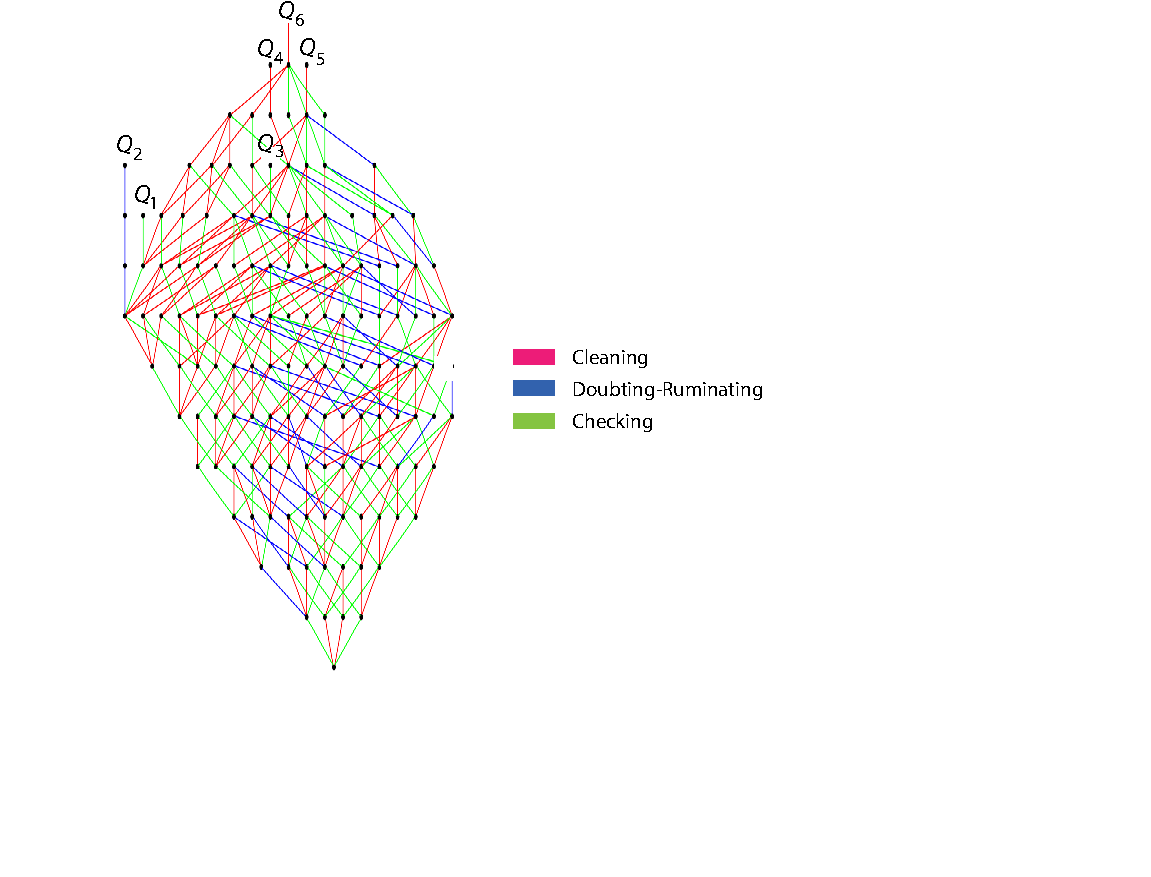
\includegraphics[scale=.70]{diagnostic_lattice_5_28_16_modified}
\end{figure}
\vspace{-5cm}

\hspace{6cm} \begin{minipage}{5cm} The color of the link indicates the symptom added to a state.
\end{minipage}
 \vspace{-1cm}

\includemedia[
  addresource=TaiwanVoiceSlide_59.mp3,
  flashvars={
    source=TaiwanVoiceSlide_59.mp3
   &autoPlay=true
  },
  transparent, passcontext
]{\fbox{Play}}{APlayer.swf}
\end{frame}


%%%%%%%%%%%%
\begin{frame}{\small The learning subspaces-syndromes induced by the maximal states\\[-.5mm]
{\footnotesize $Q_1 = \{4,7,9,10, 11,12,14,15,21\}$  \qquad\quad\qquad $Q_2 = \{2,4,5,6,10,11, 12,14,15,21\}$}\\[-2mm] Except for the top two or three symptoms  the two learning spaces are  identical.
}

\begin{figure}


\vspace{-5.5cm}


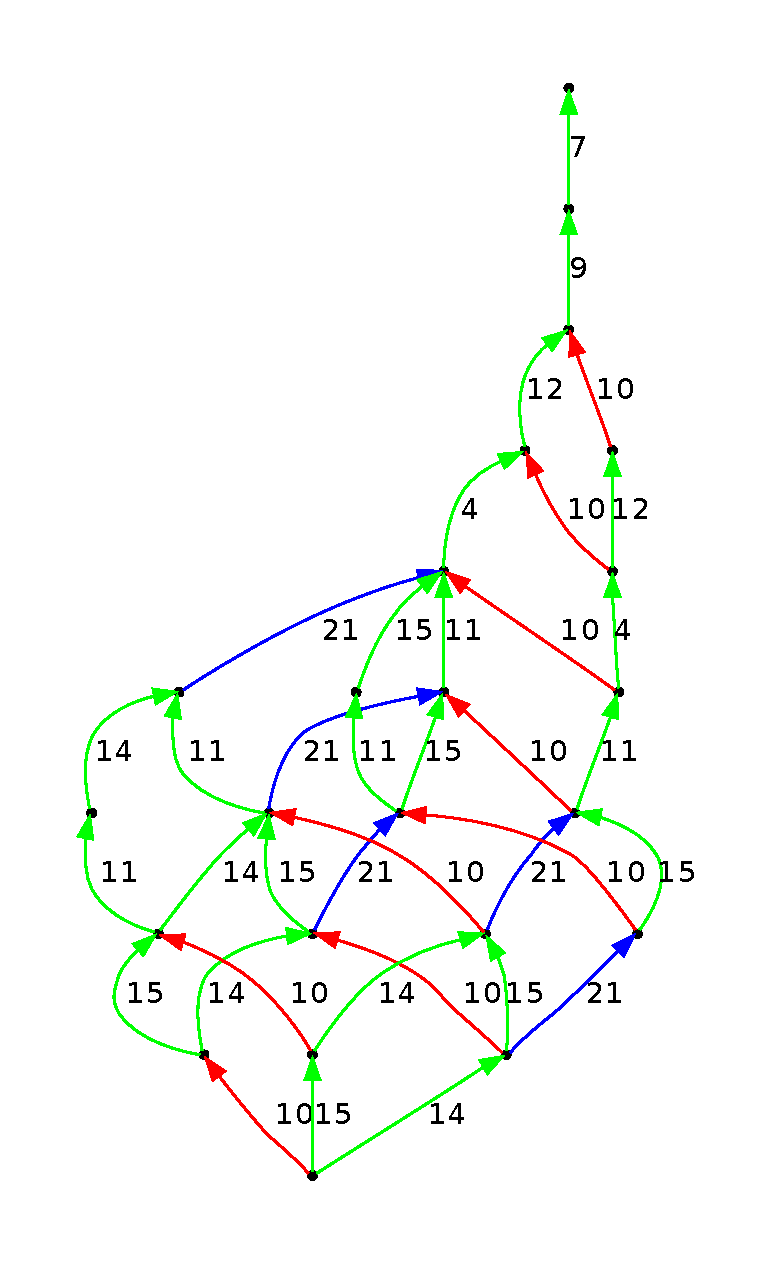
\includegraphics[scale=.38]{M1_5_28_16.pdf}
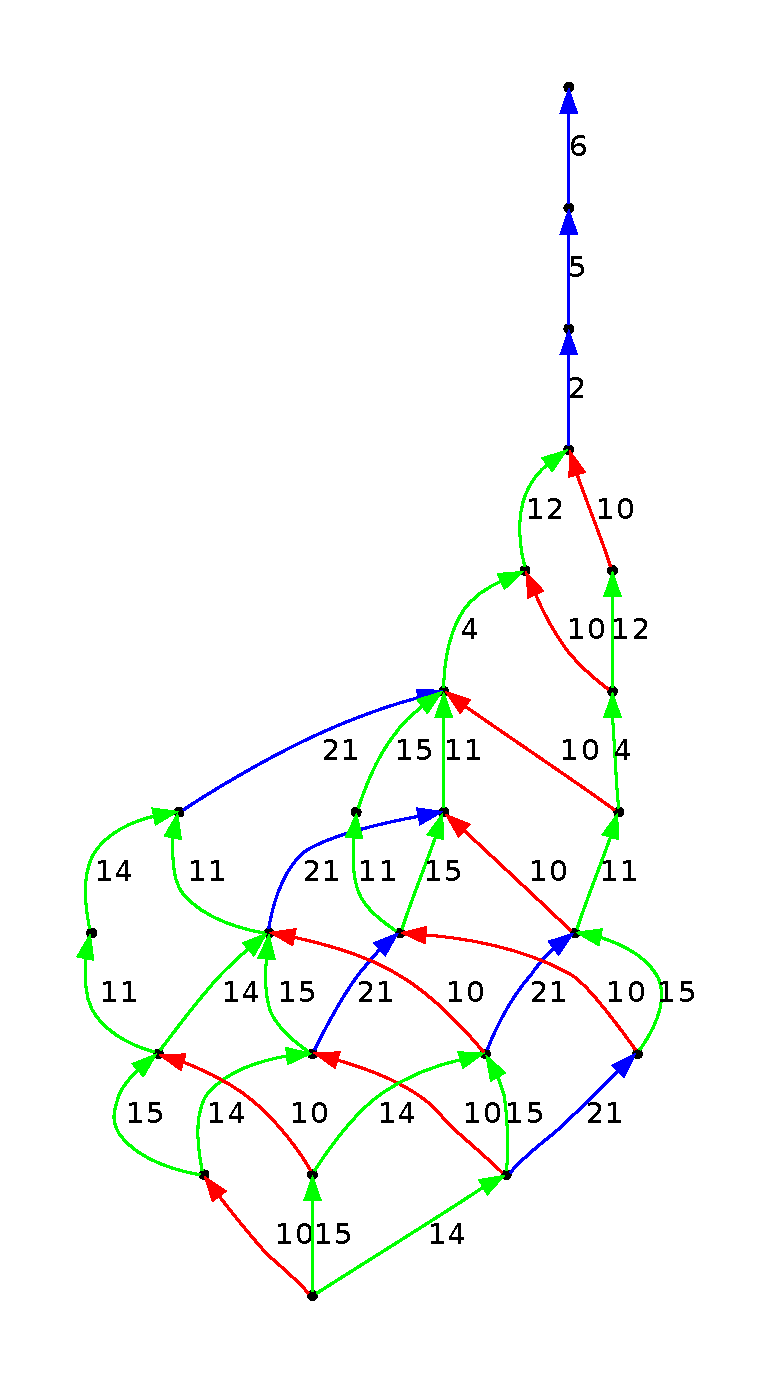
\includegraphics[scale=.36]{M2_5_28_16.pdf}

\end{figure}

%
\vspace{-8.7cm}

\hspace{9.7cm}
{\bf $Q_2$}
\vspace{-.2cm}

\hspace{4.9cm}
{\bf $Q_1$}

 \vspace{-.5cm}

\includemedia[
  addresource=TaiwanVoiceSlide_60.mp3,
  flashvars={
    source=TaiwanVoiceSlide_60.mp3
   &autoPlay=true
  },
  transparent, passcontext
]{\fbox{Play}}{APlayer.swf}
\end{frame}
%%%%%%%%%%%%
\begin{frame}{\small The syndrome induced by  $Q_3 = \{4,10,11,12,14, 15,16,19,20,21\}$}

\begin{figure}
\vspace{-5.6cm}


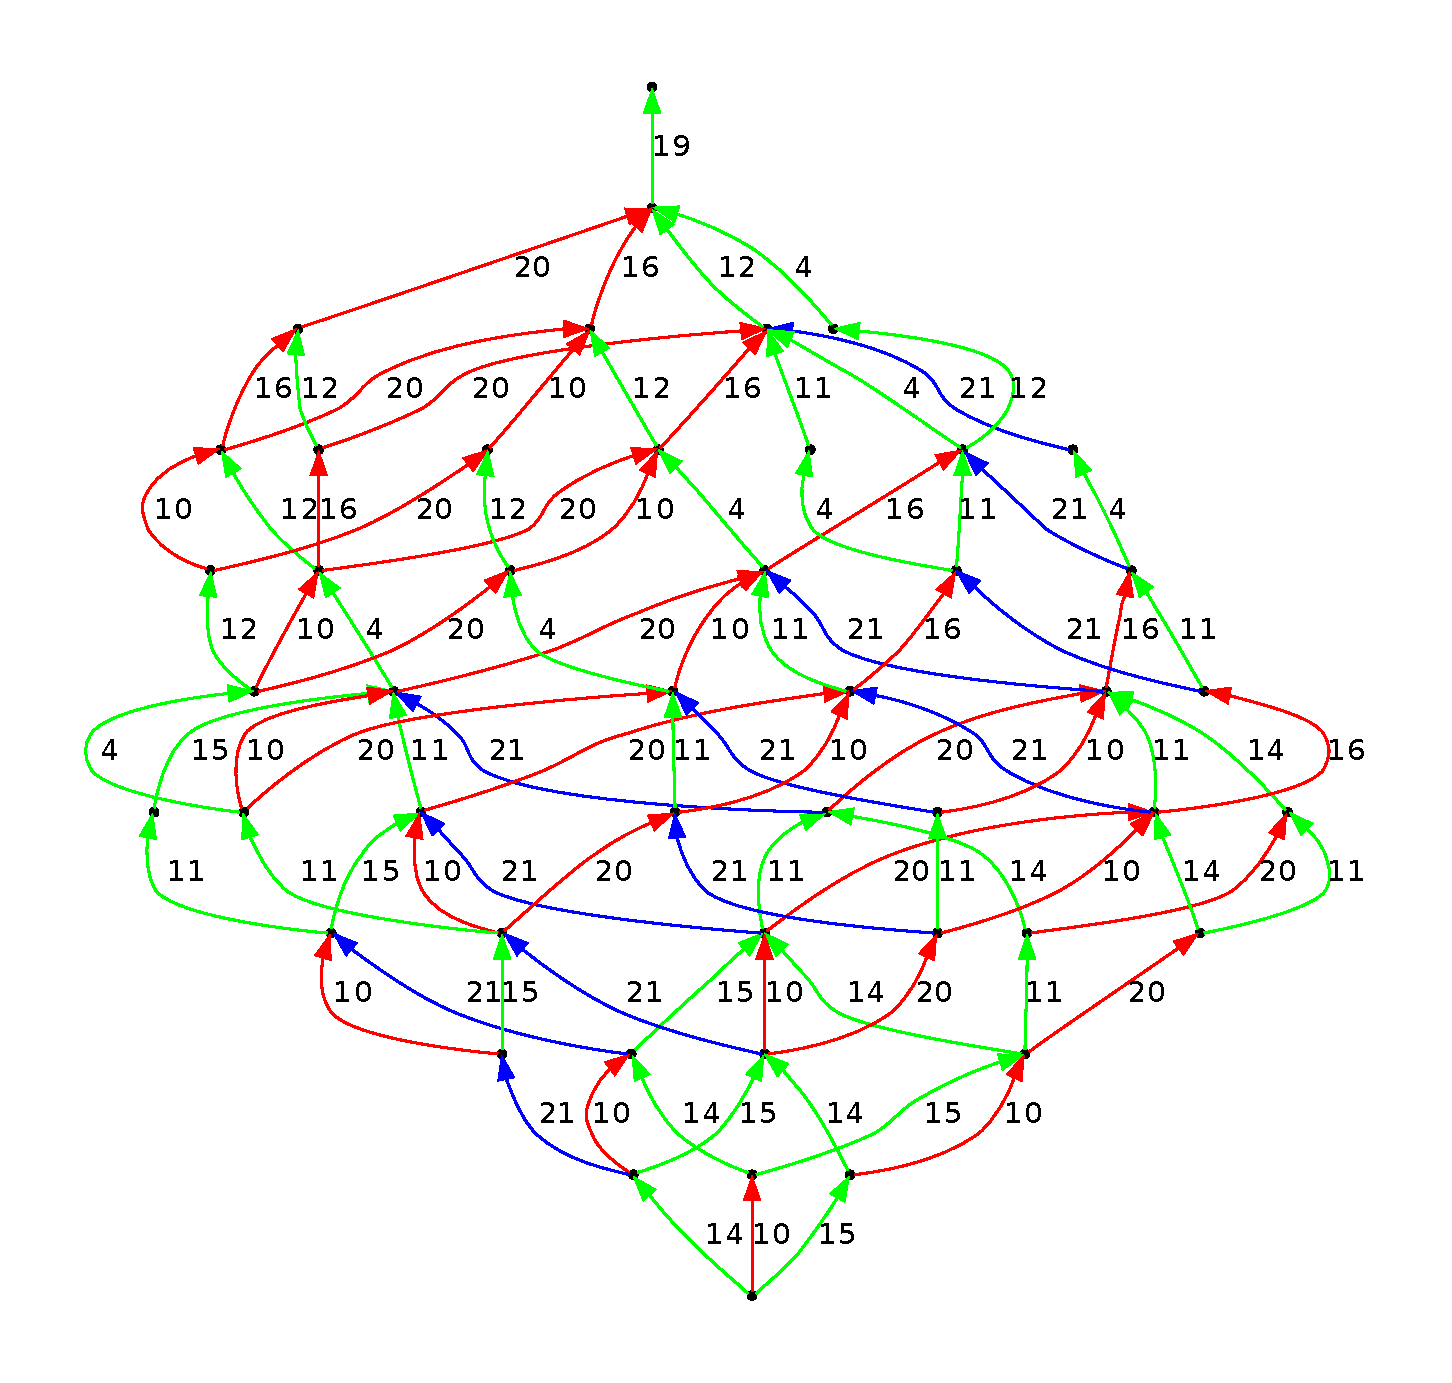
\includegraphics[scale=.38]{M3_5_28_16.pdf}
\vspace{-8.7cm}

{\bf $Q_3$}

\end{figure}
 \vspace{-.5cm}

\includemedia[
  addresource=TaiwanVoiceSlide_62.mp3,
  flashvars={
    source=TaiwanVoiceSlide_62.mp3
   &autoPlay=true
  },
  transparent, passcontext
]{\fbox{Play}}{APlayer.swf}
\end{frame}
%%%%%%%%%%%%%%%%%%%%
\begin{frame}{Comments about the loose structure.}
\center
\begin{minipage}{10.5cm} It is clear that the diagnostic space that we constructed is a rather loose structure. This is exemplified by the subspace induced by the maximal state $Q_3$\footnote{$Q_4$, $Q_5$, and $Q_6$ are even worse.}. This should not be too surprising. Examining the items of the questionnaire leads to the conclusion that few of them seem to be powerful indicators. Conceivably, some of the questions could be rephrased so as to make them more inquisitive. 
\wl
\wl
\wl
\wl
\wl
\wl
 \vspace{.5cm}

\includemedia[
  addresource=TaiwanVoiceSlide_62.mp3,
  flashvars={
    source=TaiwanVoiceSlide_62.mp3
   &autoPlay=true
  },
  transparent, passcontext
]{\fbox{Play}}{APlayer.swf}
\end{minipage}

\end{frame}
%%%%%%%%%%%%
%%%%%%%%%%%%
\begin{frame}{The stochastic assessment algorithm\\
Uncovering the current state of a patient}
\center
\begin{minipage}{10cm}
The stochastic diagnostic algorithm based on the diagnostic space theory described in this paper has much in common with that used in learning space theory.
\wl
The basic idea is obvious, which is: successively check for the presence of symptoms, with each symptom investigated depending on which symptoms have or have not been uncovered so far. However, the details are critical, and some of them may not be obvious to the practioner (such as the MD).  \end{minipage}
 \vspace{.5cm}

\includemedia[
  addresource=TaiwanVoiceSlide_63.mp3,
  flashvars={
    source=TaiwanVoiceSlide_63.mp3
   &autoPlay=true
  },
  transparent, passcontext
]{\fbox{Play}}{APlayer.swf}
\end{frame}
%%%%%%%%%%%%
\begin{frame}{The stochastic assessment algorithm\\
Uncovering the current state of a patient}

We  outline the main steps, which are based on 3 rules.
\wl
\wl

\fp
[Q] {\sc The questioning rule}\\[2mm]

\fp
[R] {\sc The response rule}\\[2mm]

\fp
[U] {\sc The updating rule}
 \vspace{.5cm}

\includemedia[
  addresource=TaiwanVoiceSlide_64.mp3,
  flashvars={
    source=TaiwanVoiceSlide_64.mp3
   &autoPlay=true
  },
  transparent, passcontext
]{\fbox{Play}}{APlayer.swf}

\end{frame}
%%%%%%%%%%%%
\begin{frame}{The stochastic assessment algorithm. First rule.}
\framesubtitle{Uncovering the current state of a patient}
\center

\begin{roster}
\item[[Q\hspace{-.18cm}]] {\sc The questioning rule.} On each step (trial) $n$ of the assessment, we assign a probability distribution $P_n$ on the set of all the states, which depends upon all the events of the previous trials. 
\end{roster}
 \vspace{.5cm}

\includemedia[
  addresource=TaiwanVoiceSlide_65.mp3,
  flashvars={
    source=TaiwanVoiceSlide_65.mp3
   &autoPlay=true
  },
  transparent, passcontext
]{\fbox{Play}}{APlayer.swf}
\end{frame}
%%%%%%%%%%%%
\begin{frame}{The stochastic assessment algorithm. First rule.}
\framesubtitle{Uncovering the current state of a patient}
\center

\begin{roster}
\item[[Q\hspace{-.18cm}]] {\sc The questioning rule.} On each step (trial) $n$ of the assessment, we assign a probability distribution $P_n$ on the set of all the states, which depends upon all the events of the previous trials. 
\wl
Initially, if we have no advance information, we suppose that all the states are equiprobable. In the case of our example:  
$$P_1(S)= \frac 1{142}\qquad\text{ for any state $S$}. 
$$
\end{roster}
\vspace{.5cm}

\includemedia[
  addresource=TaiwanVoiceSlide_66.mp3,
  flashvars={
    source=TaiwanVoiceSlide_66.mp3
   &autoPlay=true
  },
  transparent, passcontext
]{\fbox{Play}}{APlayer.swf}
\end{frame}

%%%%%%%%%%%%
\begin{frame}{The stochastic assessment algorithm. First rule.}
\framesubtitle{Uncovering the current state of a patient}
\center

\begin{roster}
\item[[Q\hspace{-.18cm}]] {\sc The questioning rule.} On each step (trial) $n$ of the assessment, we assign a probability distribution $P_n$ on the set of all the states, which depends upon all the events of the previous trials. 
\wl
Initially, if we have no advance information, we suppose that all the states are equiprobable. In the case of our example:  $P_1(S)= \frac 1{142}$ for any state $S$. 
\wl
On trial $n$ of the assessment, we  pick a \rtxt{most informative}  symptom, that is, a symptom having a current probability as close as possible to~$.5$.  (The probability of symptom $q$ on trial $n$ is the sum of the probabilities $P_n(S)$  of all the states $S$ containing $q$.)
\end{roster}
\vspace{.5cm}

\includemedia[
  addresource=TaiwanVoiceSlide_67.mp3,
  flashvars={
    source=TaiwanVoiceSlide_67.mp3
   &autoPlay=true
  },
  transparent, passcontext
]{\fbox{Play}}{APlayer.swf}
\end{frame}

%%%%%%%%%%%%
\begin{frame}{The stochastic assessment algorithm. Second rule.}
\framesubtitle{Uncovering the current state of a patient}
\center

\begin{roster}
\item[[R\hspace{-.18cm}]] {\sc The response rule.} This rule states that if a patient has some symptom $q$ which is  checked on trial $n$, this symptom  will be regarded as uncovered with some probability $1-\bb_q$. The probability $1-\bb_q$ allows for the case in which the practitioner may, for some reason or other, actually fail to detect the symptom. The probability $1-\bb_q$ may vary across symptoms. Its value for each symptom must be estimated from the data.  
\end{roster}
\vspace{.5cm}

\includemedia[
  addresource=TaiwanVoiceSlide_68.mp3,
  flashvars={
    source=TaiwanVoiceSlide_68.mp3
   &autoPlay=true
  },
  transparent, passcontext
]{\fbox{Play}}{APlayer.swf}
\end{frame}
%%%%%%%%%%%%
\begin{frame}{The stochastic assessment algorithm. Third rule.}
\framesubtitle{Uncovering the current state of a patient}
\center

\begin{roster}
\item[[U\hspace{-.18cm}]] {\sc The updating rule.} This rule specifies how the probability $P_n$ should be changed according to the events on trial $n$.  If symptom $q$ has been found to be present on trial $n$, then the probability any  state containing $q$ is increased. (Some parameters are involved here.)\\   It can be shown that this updating rule is Bayesian.  

\wl
\item[] The assessment stopped when a statistical criterion is reached, indicating that there is no informative question left to ask.
\end{roster}
\vspace{.5cm}

\includemedia[
  addresource=TaiwanVoiceSlide_69.mp3,
  flashvars={
    source=TaiwanVoiceSlide_69.mp3
   &autoPlay=true
  },
  transparent, passcontext
]{\fbox{Play}}{APlayer.swf}
\end{frame}
%%%%%%%%%%%%
\begin{frame}{A footnote: The parallel search procedure}
\center
\begin{minipage}{10cm} In some situations, there may be a large number of possible symptoms, which may result in a number of states on the\linebreak order of several millions. In such cases, a practical procedure is available\footnote{In an application of the {\sc ALEKS} system to Beginning Algebra, the assessment is based on $650$ mathematical items, and there were several millions of knowledge states. A practical assessment based on the parallel search procedure is nevertheless possible based on about 35 questions (see Falmagne et al. 2006).}, which consists in a `parallel search' in all the one-diagnostic spaces associated with each of the maximal states. 
\pha{x}

\pha{x}

\pha{x}

\end{minipage}
\vspace{.5cm}

\includemedia[
  addresource=TaiwanVoiceSlide_70.mp3,
  flashvars={
    source=TaiwanVoiceSlide_70.mp3
   &autoPlay=true
  },
  transparent, passcontext
]{\fbox{Play}}{APlayer.swf}
\end{frame}
%%%%%%%%%%%%
\begin{frame}{A footnote: The parallel search procedure}
\center
\begin{minipage}{10cm} This parallel search procedure was used in the case of our Obsessive-Compulsive Disorder situation. Ultimately the\linebreak results of the parallel search in each of the 6 one-diagnostic spaces are combined to reveal the final state. The details are in our paper\footnote{Falmagne, J.-Cl., Cosyn, E., Doble, C.W., Doignon, J.-P., and Spoto, A. {\sl From Learning Spaces to Diagnostic Spaces
with an Application to the Obsessive-Compulsive Disorder}, submitted to the Journal of Mathematical Psychology.}.
\pha{x}

\pha{x}

\pha{x}

\pha{x}

\pha{x}


\end{minipage}
\vspace{.5cm}

\includemedia[
  addresource=TaiwanVoiceSlide_71.mp3,
  flashvars={
    source=TaiwanVoiceSlide_71.mp3
   &autoPlay=true
  },
  transparent, passcontext
]{\fbox{Play}}{APlayer.swf}
\end{frame}
%%%%%%%%%%%%
\begin{frame}{Statistics of simulated assessments.}
\center
\begin{minipage}{12cm}
\includemedia[
  addresource=TaiwanVoiceSlide_72.mp3,
  flashvars={
    source=TaiwanVoiceSlide_72.mp3
   &autoPlay=true
  },
  transparent, passcontext
]{\fbox{Play}}{APlayer.swf}\hspace{2cm} {\small In the first column:\\
 $s$  is the threshold  parameter used in the stopping rule 
$| P(\AAA_q) -.5| \geq \frac s2$. If $s=0.7$, we stop the assessment when no symptom $q$ is left such that $0.15<P(\AAA_q)< 0.85$; where $P(\AAA_q)$ is the probability of all the states containing $q$;\\
$\bb$ is the probability of {\bf not} detecting a symptom $q$ when it is in the actual state.} \end{minipage}
  
\begin{center}
  \renewcommand{\arraystretch}{1.3}
\renewcommand{\tabcolsep}{.3cm}
\begin{tabular}{|c|r|c|c|} 
\hline
$(s, \beta)$&$\begin{matrix}\text{Number of}\\[-2mm]\text{questions}\end{matrix}$&
$\begin{matrix}\text{Distance between}\\[-2mm] \text{simulated state}\\[-2mm] \text{and uncovered state}\end{matrix}$&
Final entropy\\
\hline
(0.7, 0.00)&9.1 (0.92)&0.00 (0.00)&1.41 (0.56)\\
(0.7, 0.10)&9.6 (1.75)&0.29 (0.71)&1.46 (0.54)\\
(0.7, 0.15)&9.8 (2.23)&0.48 (0.88)&1.50 (0.56)\\
(0.8, 0.00)&10.3 (0.98)&0.00 (0.00)&0.97 (0.50)\\
(0.8, 0.10)&11.4 (2.18)&0.12 (0.44)&1.00 (0.52)\\
(0.8, 0.15)&12.1 (2.59)&0.29 (0.72)&1.03 (0.51)\\
\hline
\end{tabular}
 \end{center}
\end{frame}

%%%%%%%%%%%%
\begin{frame}{Statistics of simulated assessments.}
\center
\begin{minipage}{12cm}
{\bf Note that the average distance between the simulated state and the uncovered state is less that half a symptom in all six cases.\linebreak The numbers are in red. In fact, the distance is zero in two cases.}
\end{minipage}
 \wl 
\begin{center}
  \renewcommand{\arraystretch}{1.3}
\renewcommand{\tabcolsep}{.3cm}
\begin{tabular}{|c|r|c|c|} 
\hline
$(s, \beta)$&$\begin{matrix}\text{Number of}\\[-2mm]\text{questions}\end{matrix}$&
$\begin{matrix}\text{Distance between}\\[-2mm] \text{simulated state}\\[-2mm] \text{and uncovered state}\end{matrix}$&
Final entropy\\
\hline
(0.7, 0.00)&9.1 (0.92)&\rtxt{\bf 0.00} (0.00)&1.41 (0.56)\\
(0.7, 0.10)&9.6 (1.75)&\rtxt{\bf 0.29} (0.71)&1.46 (0.54)\\
(0.7, 0.15)&9.8 (2.23)&\rtxt{\bf 0.48} (0.88)&1.50 (0.56)\\
(0.8, 0.00)&10.3 (0.98)&\rtxt{\bf 0.00} (0.00)&0.97 (0.50)\\
(0.8, 0.10)&11.4 (2.18)&\rtxt{\bf 0.12} (0.44)&1.00 (0.52)\\
(0.8, 0.15)&12.1 (2.59)&\rtxt{\bf 0.29} (0.72)&1.03 (0.51)\\
\hline
\end{tabular}
 \end{center}
 \vspace{.2cm}

\includemedia[
  addresource=TaiwanVoiceSlide_73.mp3,
  flashvars={
    source=TaiwanVoiceSlide_73.mp3
   &autoPlay=true
  },
  transparent, passcontext
]{\fbox{Play}}{APlayer.swf}
\end{frame}
%%%%%%%%%%%%%%%%%%
\begin{frame}{One objection: The disappearing symptoms}

\center
\begin{minipage}{11.5cm}
A symptom pointing  to a disease at an early stage of an ailment may disappear  later on in the evolution of the disease, as in the case of the {\sl Lyme disease}. So, the full set of symptoms discernible  at a late stage of a disease may not contain all the symptoms that have appeared in the course of the disease. 
\end{minipage}
\vspace{1cm}

\includemedia[
  addresource=TaiwanVoiceSlide_74.mp3,
  flashvars={
    source=TaiwanVoiceSlide_74.mp3
   &autoPlay=true
  },
  transparent, passcontext
]{\fbox{Play}}{APlayer.swf}
\end{frame}
%%%%%%%%%%%%
\begin{frame}{One objection: The disappearing symptoms}
\center
\begin{minipage}{10.5cm}

\begin{examplelyme}\sl\small ``Lyme disease is an infection resulting from the bite of deer ticks carrying a particular bacterium. According to the Centers for Disease Control and Prevention, there are about $329,000$ cases of Lyme disease annually in the U.S. 
\tl
An early symptom of the disease is rash. The infection spreads gradually around the site of the tick bite. The rash begins about a week after the bite, and will usually disappear in about a month. However, the bacteria responsible for the infection may remain inside the body. If the patient is not treated right away, other symptoms will appear, as the bacteria spread from the skin to the blood stream\footnote{See The Merck Manual, 1999, pages 1189-1191.}.''  
\end{examplelyme} 
\end{minipage}
\vspace{.5cm}

\includemedia[
  addresource=TaiwanVoiceSlide_75.mp3,
  flashvars={
    source=TaiwanVoiceSlide_75.mp3
   &autoPlay=true
  },
  transparent, passcontext
]{\fbox{Play}}{APlayer.swf}
\end{frame}
%%%%%%%%%%%%
\begin{frame}{The disappearing symptoms and the cured symptoms}

\center
\begin{minipage}{10.5cm}
The way we could  deal with the disappearance of some symptom $q$ is via the occurrence of a `disappearing indicator' $\bar q$ occurring later, which would have, from the standpoint of the theory,  the status of a new symptom.
\wl
But even if we adequately handle the disappearing symptoms in this fashion, the picture may not be complete because we may still have to take care of symptoms disappearing because they are  `{cured}', which would lead to the concept of a `{cured state}.' 
\end{minipage}
\vspace{.5cm}

\includemedia[
  addresource=TaiwanVoiceSlide_76.mp3,
  flashvars={
    source=TaiwanVoiceSlide_76.mp3
   &autoPlay=true
  },
  transparent, passcontext
]{\fbox{Play}}{APlayer.swf}
\end{frame}
%%%%%%%%%%%%
\begin{frame}{The cured symptoms}
\center
\begin{minipage}{10.5cm} Mimicking the device used for the disappearing symptoms, we will  symbolize a cured symptom $q$ by a `cured indicator' $\curedq$, also to be taken as a new symptom. 
\end{minipage}
\vspace{.5cm}

\includemedia[
  addresource=TaiwanVoiceSlide_77.mp3,
  flashvars={
    source=TaiwanVoiceSlide_77.mp3
   &autoPlay=true
  },
  transparent, passcontext
]{\fbox{Play}}{APlayer.swf}
\end{frame}
%%%%%%%%%%%%%
\begin{frame}
\center
\frametitle{An example of a diagnostic space with two syndromes}
\vspace*{-.5cm}

\hspace{-6cm}
\begin{minipage}{6.6cm}\small
\pha{xxx}The symptoms are $a$, $b$, $c$ and $d$.
\hspace{-.3cm}
\begin{roster}
\itbul $b$ is a disappearing symptom in the syndrome
on the left, and a curable symptom
in the syndrome on the right;
\vspace{-.2cm}

\itbul $a$ is disappearing on the right.
\end{roster}
\end{minipage}
\begin{center}
\vspace{-2.3cm}

\hspace*{-1cm}
{\scriptsize
\begin{tikzpicture}[scale= .4]   
       \node [ellipse,draw] at (9,-8) (b) {$\{b\}$};
       \node at (5,-8) {$\begin{smallmatrix}\text{\rtxt{the disappearing}}\\ \text{\rtxt{symptom $b$ occurs}}\end{smallmatrix}$}; 
       \node at (26,-8) {$\begin{smallmatrix}\text{\rtxt{the disappearing}}\\ \text{\rtxt{symptom $a$ occurs}}\end{smallmatrix}$};   
      \node at (22,-5.3) {$\begin{smallmatrix}\text{\rtxt{$a$ disappears} $\nearrow$}\\ \swarrow\rtxt{\text{marked by $\bar a$}}\end{smallmatrix}$};    
          \node [ellipse,draw] at (22,-8) (a) {$\{a\}$};
             \node [ellipse,draw] at (9,-4.5) (bc) {$\{b,c\}$};
              \node [ellipse,draw] at (26,-5.5) (ab) {$\{a,b\}$};
               \node [ellipse,draw] at (18,-5.5) (abar a) {$\{a,\bar a\}$};
                \node [ellipse,draw] at (4,-1.5) (bbar bc) {$\{b,\bar b, c\}$};
                 \node [ellipse,draw] at (14,-1.5) (bcd) {$\{b,c,d\}$};
                      \node at (9,-1.5) {$\begin{smallmatrix}\text{\rtxt{$b$ disappears} $\nearrow$}\\ \swarrow\rtxt{\text{marked by $\bar b$}}\end{smallmatrix}$}; 
  \node [ellipse,draw] at (22,-3) (abar ab) {$\{a,\bar a,b\}$};
                  \node [ellipse,draw] at (22,.1) (abar abe) {$\{a,\bar a,b,e\}$};
                     \node [ellipse,draw] at (10,2) (bbar bcd) {$\{b,\bar b,c,d\}$
                     $\begin{smallmatrix}\text{incurable}\\ \text{disease}\end{smallmatrix}$};
                       \node [ellipse,draw] at (22,3.5) (abar a curedb e) {$\{a,\bar a,b,\curedb,e\}$};
                        \node [ellipse,draw] at (22,7.3) (abar a curedb curede) {$\{a,\bar a,b,\curedb,e,\curede\}$$\begin{smallmatrix}\text{cured}\\ \text{disease}\end{smallmatrix}$};                       
                                                             
             \node [ellipse,thick, draw] at (15,-9.7) (es) {$\es$};
%
%
\path[-] (es) edge node [below right] {$a$} (a);
\path[-] (es) edge node [below left] {$b$} (b);
\path[-] (b) edge node [right] {$c$} (bc);
\path[-] (a) edge node [below left] {$\bar a$} (abar a);
\path[-] (a) edge node [right] {$b$} (ab);
\path[-] (bc) edge node [below left] {$\bar b$} (bbar bc);
\path[-] (bc) edge node [right] {$d$} (bcd);
\path[-] (abar a) edge node [above left] {$b$} (abar ab);
\path[-] (ab) edge node [above] {\pha{x}$\bar a$} (abar ab);
\path[-] (bbar bc) edge node [right] {$d$} (bbar bcd);
\path[-] (bcd) edge node [right] {\pha{i}$\bar b$} (bbar bcd);
\path[-] (abar ab) edge node [right] {$e$} (abar abe);
\path[-] (abar abe) edge node [right] {$\curedb \,\,\,\,\leftarrow \begin{matrix} \rtxt{b \text{ is cured}}\end{matrix}$} (abar a curedb e);
\path[-] (abar a curedb e) edge node [right] {$\curede \,\,\,\,\leftarrow \begin{matrix} \rtxt{e \text{ is cured}}\end{matrix}$} (abar a curedb curede);

\end{tikzpicture}
}
\end{center}
\vspace{-.7cm} 

\hspace{-7.5cm}
\includemedia[
  addresource=TaiwanVoiceSlide_78.mp3,
  flashvars={
    source=TaiwanVoiceSlide_78.mp3
   &autoPlay=true
  },
  transparent, passcontext
]{\fbox{Play}}{APlayer.swf}
\end{frame}
%%%%%%%%%%%%
\begin{frame}
\frametitle{Other algorithmic softwares for medical diagnosis.}
\center
\begin{minipage}{10.5cm} Existing medical diagnosis software falls under the term: 
\tl
\centerline{``{\sl Clinical diagnosis support systems}'' (CDSS).}
\tl

They tend to be based on very different principles. 
\tl
Three examples.
\begin{roster}
\itbul {\bf DXplain}, developed by the Massachussets General Hospital has a data base of about $230,000$ disease-symptom pairs and uses a Bayesian approach.
\itbul {\bf Isabel}, developed privately in the UK is also based on Bayesian principles.
\itbul {\bf IBM Watson} uses powerful search algorithms and access to large amount of information to generate and test hypotheses and rank results (again using Bayesian principles).
\end{roster} 
\end{minipage}
\includemedia[
  addresource=TaiwanVoiceSlide_79.mp3,
  flashvars={
    source=TaiwanVoiceSlide_79.mp3
   &autoPlay=true
  },
  transparent, passcontext
]{\fbox{Play}}{APlayer.swf}
\end{frame}
%%%%%%%%%%%%
\begin{frame}
\frametitle{Final Note}
\vspace{1cm}
\center
\begin{minipage}{9.8cm}  
 As far as we can tell from their descriptions, these other medical diagnosis softwares are based on psychometric principles quite different from the stochastic-combinatoric framework that I have described. For example, none of them is equipped with the joint concepts of inner/outer fringes.
\end{minipage}
\vspace{.5cm}

\includemedia[
  addresource=TaiwanVoiceSlide_80.mp3,
  flashvars={
    source=TaiwanVoiceSlide_80.mp3
   &autoPlay=true
  },
  transparent, passcontext
]{\fbox{Play}}{APlayer.swf}
\end{frame}

%%%%%%%%%%%%
\begin{frame}
\frametitle{Final Note}
\vspace{1cm}
\center
\begin{minipage}{9.2cm}  In the application of the Obsessive-Compulsive disorder that we described, all the symptoms were clinical, of the psychiatric type.
\tl
But it should be clear that the Diagnostic Space theory is applicable with any kind of symptoms, including for example, a symptom uncovered by neur 
\tl
 In fact, the carefully monitored assessment sequence of the symptoms is especially useful when the assessment may be  expensive. In this case, it is essential that the each symptom verification is most informative, e.g.~in the sense that I have discussed.
\end{minipage}
\vspace{.5cm}

\includemedia[
  addresource=TaiwanVoiceSlide_81.mp3,
  flashvars={
    source=TaiwanVoiceSlide_81.mp3
   &autoPlay=true
  },
  transparent, passcontext
]{\fbox{Play}}{APlayer.swf}

\end{frame}


%%%%%%%%%%%%
\begin{frame}
\vspace{1cm}
\center

{\Large  THANK YOU\,\,!}
\vspace{1cm}

\includemedia[
  addresource=TaiwanVoiceSlide_82.mp3,
  flashvars={
    source=TaiwanVoiceSlide_82.mp3
   &autoPlay=true
  },
  transparent, passcontext
]{\fbox{Play}}{APlayer.swf}

\end{frame}
%%%%%%%%%%%%
%\begin{frame}
%
%\center
%\begin{tikzpicture}[scale= .33]   
%
%                 \node [draw] at (11.7,-3.2) (b) {$b$};
%              \node [draw] at (15,-4) (f) {$f$};
%                   \node [draw] at (15,-1) (e) {$e$};
%                       \node [draw] at (13,2) (h) {$h$};
%                        \node [draw] at (17,2) (i) {$i$};
%                        \node [draw] at (15,5.3) (j) {$j$};       
%                          \node [draw] at (7.9,-.5) (c) {$c$};  
%                           \node [draw] at (15,-7) (a) {$a$}; 
%                           \node [red,draw] at (10,2) (d) {$d$}; 
%                           \node [red,draw] at (4,2) (g) {$g$};                
%%
%\draw[<-, thick] (e)--(b);
%\draw[<-, thick] (j)--(h);
%\draw[<-, thick] (j)--(i);
%\draw[<-, thick] (i)--(e);
%\draw[<-, thick] (h)--(e);
%\draw[<-, thick] (e) --(f);
%\draw[<-, thick] (f) --(a);
%\draw[<-, thick] (c) --(b);
%\draw[<-, thick] (g) --(c);
%\draw[<-, thick] (d) --(c);
%                           \draw [ very thick, rotate=-35] (7.2, 3.9) ellipse (6cm and 2.5cm); %%%% Q1   
%                            \draw [ very thick, rotate=81] (1.8, -15.7) ellipse (7.5cm and 5cm); %%% Q2 
%                             \draw [ very thick, rotate=81] (0, -10) ellipse (4.5cm and 3cm); %%%Q3 
%                             
%                            \node[rounded rectangle, draw, fill=white!100] at (13,9) (Q2) 
%                            {$\footnotesize Q_2=\{j,i,h,e,b,f,a\}$};
% \draw[thick,->] (Q2)--(15,6.5); 
%                            \node[rounded rectangle, draw, fill=white!100] at (2,4.5) (Q1) 
%                            {$\footnotesize Q_1=\{b,c,g\} $};
% \draw[thick,->] (Q1)--(3.7,2.9);   
% \node[rounded rectangle, draw, fill=white!100] at (3,-6) (Q3) 
%                            {$\footnotesize Q_3=\{b,c,d\} $};
% \draw[thick,->] (Q3)--(7.5,-5);     
%%
%
%
%\end{tikzpicture}
%\end{frame}
%\begin{frame}
%{\sc \small The definition of a diagnostic space does not change.\\[-2mm] We only have to define the set of critically defining symptoms.}
%
%\begin{tikzpicture}[scale= .35]   
%
%                 \node [draw] at (11.7,-3.2) (b) {$b$};
%              \node [draw] at (15,-4) (f) {$f$};
%                   \node [draw] at (15,-1) (e) {$e$};
%                       \node [draw] at (13,2) (h) {$h$};
%                        \node [draw] at (17,2) (i) {$i$};
%                        \node [draw] at (15,5.3) (j) {$j$};       
%                          \node [draw] at (7.9,-1.8) (c) {$c$};  
%                           \node [draw] at (15,-7) (a) {$a$}; 
%                           \node [red,draw] at (10.2,1.7) (d) {$d$}; 
%                           \node [draw] at (5,1) (k) {$k$};   
%                            \node [red,draw] at (2.5,3) (g) {$g$};               
%%
%\draw[<-, thick] (e)--(b);
%\draw[<-, thick] (j)--(h);
%\draw[<-, thick] (j)--(i);
%\draw[<-, thick] (i)--(e);
%\draw[<-, thick] (h)--(e);
%\draw[<-, thick] (e) --(f);
%\draw[<-, thick] (f) --(a);
%\draw[<-, thick] (c) --(b);
%\draw[<-, thick] (k) --(c);
%\draw[<-, thick] (d) --(c);
%\draw[<-, thick] (g) --(k);
%                           \draw [ very thick, rotate=-34] (5.9, 3.4) ellipse (7.2cm and 2.5cm); %%%% Q1   
%                            \draw [ very thick, rotate=81] (1.8, -15.7) ellipse (7.5cm and 5cm); %%% Q2 
%                             \draw [ very thick, rotate=81] (0, -10) ellipse (4.5cm and 3cm); %%%Q3 
%                             
%                            \node[rounded rectangle, draw, fill=white!100] at (13,9) (Q2) 
%                            {$\footnotesize Q_2=\{j,i,h,e,b,f,a\}$};
% \draw[thick,->] (Q2)--(15,6.5); 
%                            \node[rounded rectangle, draw, fill=white!100] at (2,7) (Q1) 
%                            {$\footnotesize Q_1=\{b,c,k,g\} $};
% \draw[thick,->] (Q1)--(2.5,4.1);   
% \node[rounded rectangle, draw, fill=white!100] at (5.5,-7.5) (Q3) 
%                            {$\footnotesize Q_3=\{b,c,d\} $};
% \draw[thick,->] (Q3)--(7.6,-5);     
%%
%
%
%\end{tikzpicture}
%
%\end{frame}
%
%\begin{frame}
%
%\frametitle{\small Tentative conditions on a set of critically defining symptoms}
%
%\begin{definition}\label{def_diag_space_CD} Suppose that $(\QQQ,\AAA)$ is a diagnostic space, with $\QQQ=\{Q_1,\ldots,Q_N\}$ and $Q= \cup_{1\leq i\leq N}Q_i$. A set  of symptoms $Q^*$ is a {\sl set of critically defining symptoms consistent} with the diagnostic space $(\QQQ,\AAA)$ if it satisfies the three conditions below: 
%\begin{roster}
%\item $Q^*\subset Q$;
%\item any symptom in $Q^*$ is a maximal symptom of $(\QQQ,\AAA)$ in the sense of our definition; 
%\item  for any two distinct maximal states $Q_i, Q_j\in\AAA$, we have $Q_i\cap Q_j\cap Q^*=\es$.
%\end{roster}
%\end{definition}
%
%{\small Thus, Condition 3 requires that any CD symptom belongs to at most one maximal state.  On the other hand, there may be more than one CD symptom in any maximal state. }  
%\end{frame}

 \end{document}
